\chapter[Basic Data Representation]{Basic Data\\ Representation}
\label{chap:basic_data_representation}

% Position the image to the right of the heading.
\vspace{-9\baselineskip} % move up
\hfill
 \begin{minipage}{0.5\textwidth}
 \centering
 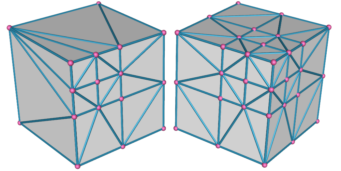
\includegraphics{VTKTextbook-48}
  \captionof*{figure}{\textit{Compatible tessellations.}}
 \end{minipage}
\vspace{2\baselineskip}

\firstletter{I}n Chapter 4 we developed a pragmatic definition of the visualization process: mapping information into graphics primitives.
We saw how this mapping proceeds through one or more steps, each step transforming data from one form, or data representation, into another.
In this chapter we examine common data forms for visualization.
The goal is to familiarize you with these forms, so that you can visualize your own data using the tools and techniques provided in this text.

\section{Introduction}
To design representational schemes for data we need to know something about the data we might
encounter. We also need to keep in mind design goals, so that we can design efficient data structures
and access methods. The next two sections address these issues.

\subsection{Characterizing Visualization Data}

Since our aim is to visualize data, clearly we need to know something about the character of the data. This knowledge will help us create useful data models and powerful visualization systems. Without a clear understanding of the data, we risk designing inflexible and limited visualization systems. In the following we describe important characteristics of data. These characteristics are the discrete nature of data\index{discrete data}, whether it is regular or irregular, and its topological dimension.

First, visualization data is discrete. This is because we use digital computers to acquire, analyze, and represent our data, and typically measure or sample information at a finite number of points. Hence, all information is necessarily represented in discrete form. 

Consider visualizing the simple continuous function $y = x6 2$. If we are using a conventional digital computer, we must discretize this equation to operate on the data it represents (we are ignoring symbolic/analog computers and methods.) For example, to plot this equation we would sample the function in some interval, say $(-1,1)$, and then compute the value y of the function at a series of discrete points $x = x_i$ in this interval. The resulting points $((x_0,y_0), (x_1,y_1), (x_2,y_2), ... (x_n,y_n))$ connect the points with straight line segments. Thus, our (continuous) data is represented by a discrete sampling.

Because of the discrete character of the data we do not know anything about regions in between data values. In our previous example, we know that data is generated from the function $y = x^2$, but, generally speaking, when we measure and even compute data, we cannot infer data values between points. This poses a serious problem, because an important visualization activity is to determine data values at arbitrary positions. For example, we might probe our data and desire data values even though the probe position does not fall on a known point.

There is an obvious solution to this problem: interpolation. We presume a relationship between neighboring data values. Often this is a linear function, but we can use quadratic, cubic, spline, or other interpolation functions. Chapter 8: \nameref{chap:advanced_data_representation} discusses interpolation functions in greater detail, but for now suffice it to say that interpolation functions generate data values in between known points.

A second important characteristic of visualization data is that its structure may be regular or irregular (alternatively, structured or unstructured). Regular data has an inherent relationship between data points. For example, if we sample on an evenly spaced set of points, we do not need to store all the point coordinates, only the beginning position of the interval, the spacing between points, and the total number of points. The point positions are then known implicitly, which can be taken of advantage of to save computer memory.

Data that is not regular is irregular data. The advantage of irregular data is that we can represent information more densely where it changes quickly and less densely where the change is not so great. Thus, irregular data allows us to create adaptive representational forms, which can be beneficial given limited computing resources.

Characterizing data as regular or irregular allows us to make useful assumptions about the data. As we saw a moment ago, we can store regular data more compactly. Typically, we can also compute with regular data more efficiently relative to irregular data. On the other hand, irregular data gives us more freedom in representing data and can represent data that has no regular patterns.

Finally, data has a topological dimension. In our example $y = x^2$ , the dimension of the data is one, since we have the single independent variable $x$. Data is potentially of any dimension from 0D points, to 1D curves, 2D surfaces, 3D volumes, and even higher dimensional regions.

The dimension of the data is important because it implies appropriate methods for visualization and data representation. For example, in 1D we naturally use x-y plots, bar charts, or pie charts, and store the data as a 1D list of values. For 2D data we might store the data in a matrix, and visualize it with a deformed surface plot (i.e., a \emph{height field}\index{height field} --- see Exercise 2 on page \pageref{ex:ch04_4.2}).

In this chapter and Chapter 8: \nameref{chap:advanced_data_representation}, we show how these characteristics: discrete, regular/irregular, and data dimension, shape our model of visualization data. Keep these features in mind as you read these chapters.

\begin{figure}[!htb]
	\centering
	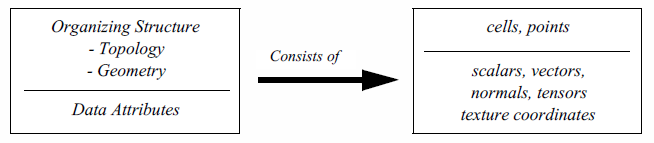
\includegraphics[width=0.8\textwidth]{Figure5-1}
	\caption{The architecture of a dataset. A dataset consists of an organizing structure, with both topological and geometric properties, and attribute data associated with the structure.}
	\label{fig:Figure5-1}
\end{figure}

\subsection{Design Criterion}

Visualizing data involves interfacing to external data, mapping into internal form, processing the data, and generating images on a computer display device. We pose the question: What form or forms should we use to represent data? Certainly many choices are available to us. The choice of representation is important because it affects the ability to interface to external data and the performance of the overall visualization system. To decide this issue we use the following design criteria:

\begin{description}

\item[Compact.] Visualization data tends to be large, so we need compact storage schemes to minimize computer memory requirements.

\item[Efficient.] Data must be computationally accessible. We want to retrieve and store data in constant time (i.e., independent of data size). This requirement offers us the opportunity to develop algorithms that are linear, or $O(n)$, in time complexity.

\item[Mappable.] There are two types of mappings. First, data representations need to efficiently map into graphics primitives. This ensures fast, interactive display of our data. Second, we must be able to easily convert external data into internal visualization data structures. Otherwise, we suffer the burden of complex conversion processes or inflexible software

\item[Minimal Coverage.] A single data representation cannot efficiently describe all possible data types. Nor do we want different data representations for every data type we encounter. Therefore, we need a minimal set of data representations that balances efficiency against the number of data types.

\item[Simple.] A major lesson of applied computation is that simple designs are preferable to complex designs. Simple designs are easier to understand, and therefore, optimize. The value of simplicity cannot be overemphasized. Many of the algorithms and data representations in this text assign high priority to this design criterion.

\end{description}

The remainder of this chapter describes common visualization data forms based on these design criteria. Our basic abstraction is the \emph{data object}\index{data object}, a general term for the various concrete visualization data types which are the subclasses of data object. 

\section{The Data Object}

The most general form of data found in VTK is the data object\index{data object}. A data object can be thought of as a collection of data without any form. Data objects represent the data that is processed by the visualization pipeline (see the previous chapter and Figure \ref{fig:Figure4-2}). Taken by themselves, data objects carry little useful information. It is only when they are organized into some structure that they provide a form that we can operate on with visualization algorithms.

\section{The Dataset}
\label{sec:dataset}
\index{dataset|(}\index{geometry!dataset|(}

Data objects with an organizing structure and associated data attributes (Figure \ref{fig:Figure5-11}) form datasets. The dataset is an abstract form; we leave the representation\index{cell!representation} and implementation of the structure to its concrete subclasses. Most algorithms (or process objects) in VTK operate on datasets.

The structure has two parts: topology and geometry. Topology\index{dataset!topology} is the set of properties invariant under certain geometric transformations \cite{Weiler86}. Here we consider the transformations: rotation, translation, and nonuniform scaling. Geometry\index{dataset!geometry} is the instantiation of the topology, the specification of position in 3D space. For example, saying that a polygon is a ``triangle'', specifies topology. By providing point coordinates, we specify geometry.

Dataset attributes are supplemental information associated with geometry and/or topology. This information might be a temperature value at a point or the inertial mass of a cell.

Our model of a dataset assumes that the structure consists of cells and points. The cells specify the topology, while the points specify the geometry. Typical attributes include scalars, vectors, normals, texture coordinates, and tensors.

The definition of the structure of a dataset as a collection of cells and points is a direct consequence of the discrete nature of our data. Points are located where data is known and the cells allow us to interpolate between points. We give detailed descriptions of dataset structure and attributes in the following sections.
\index{dataset|)}\index{geometry!dataset|)}

\section{Cell Types}
\label{sec:cell_types}
\index{cell|(}

A dataset consists of one or more cells (Figure \ref{fig:Figure5-2} and Figure \ref{fig:Figure5-4}). Cells are the fundamental building blocks of visualization systems. Cells are defined by specifying a type in combination with an ordered list of points. \index{cell!as topology}The ordered list, often referred to as the \emph{connectivity list}\index{connectivity list}, combined with the type specification, implicitly defines the topology of the cell. The $x-y-z$ point coordinates define the cell geometry.

Figure \ref{fig:Figure5-3} shows one cell type, a hexahedron. The ordered list is a sequence of point ids that index into a point coordinate list. The topology of this cell is implicitly known: we know that $(8,10)$ is one of the 12 edges of the hexahedron, and that $(8,10,22,21)$ is one of its six faces.

Mathematically, we represent a cell by the symbol $C_i$. Then the cell is an ordered set of points $C_1 = {p_1, p_2,..., p_n}$ with $p_i \in P$ is a set of n-dimensional points (here $n=3$). They type of cell determines the sequence of points or cell topology. The number of points $n$ defining the cell is the \emph{size} of the cell. A cell $C_i$ ``uses'' a point $p_i$ when $p_i \in C_i$. Hence the ``use set'' $U(p_i)$ is the collection of all cells using $p_i$:

\begin{equation}\label{eq:5.1}
U(p_i) = {C_i:p_i \in C_i}
\end{equation}
\myequations{The ``use set''. }

\begin{figure}[!htb]
	\centering
	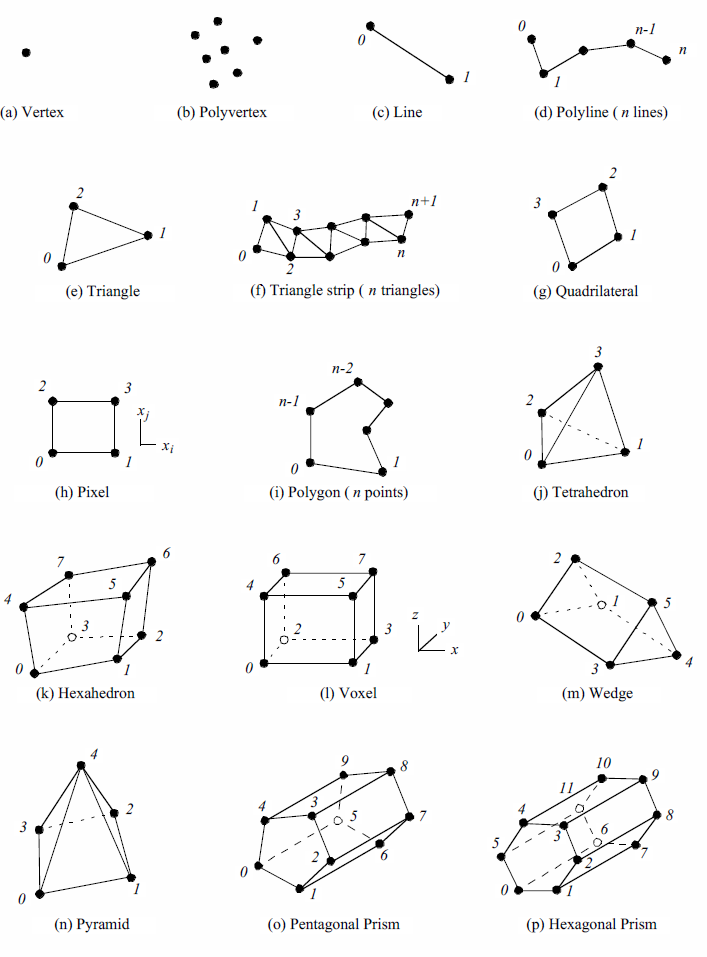
\includegraphics[width=0.8\textwidth]{Figure5-2}
	\caption{Linear cell types found in VTK. Numbers define ordering of the defining points.}
	\label{fig:Figure5-2}
\end{figure}


\begin{figure}[!htb]
	\centering
	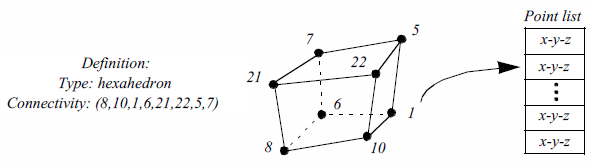
\includegraphics[width=0.8\textwidth]{Figure5-3}
	\caption{Example of a hexahedron cell. The topology is implicitly defined by the ordering of the point list. Physical generation of an image.}
	\label{fig:Figure5-3}
\end{figure}

The importance of ``uses'' and ``use sets'' will become evident in Chapter 8: \nameref{chap:advanced_data_representation} when we explore the topology of datasets.

Although we define points in three dimensions, cells may vary in topological dimension. Vertices, lines, triangles, and tetrahedron are examples of topologically 0, 1, 2, and 3--D cells, respectively, embedded in three-dimensional geometric space. Cells can also be primary or composite. Composite\index{cell!composite}\index{composite cell} cells consist of one or more primary cells, while primary\index{cell!primary} cells cannot be decomposed into combinations of other primary cell types. A triangle strip, for example, consists of one or more triangles arranged in compact form. The triangle strip is a composite cell because it can be broken down into triangles, which are primary cells.

Certainly there are an infinite variety of possible cell types. In the \emph{Visualization Toolkit} each cell type has been chosen based on application need. We have seen how some cell types: vertex, line, polygon, and triangle strip (\ref{fig:Figure3-19}) are used to represent geometry to the graphics subsystem or library. Other cell types such as the tetrahedron and hexahedron are common in numerical simulation. The utility of each cell type will become evident through the practice of visualization throughout this book. A description of the cell types found in the \emph{Visualization Toolkit} including their classification as linear, nonlinear, or other is given in the following sections.

\subsection{Linear Cells}

Linear cells are characterized by linear or constant interpolation functions (see ``Interpolation Functions'' on page \pageref{sec:interpolation_functions} for more information). As a result, cells of dimension one or greater are characterized by straight edges. Thus any edge may be characterized by two vertex id 's $(v1,v2)$. The following are the linear cells currently found in VTK.

\begin{description}

\item[Vertex.\index{cell!vertex}] The vertex is a primary\index{cell!primary} zero--dimensional cell. It is defined by a single point.

\item[Polyvertex.\index{cell!polyvertex}] The polyvertex is a composite\index{cell!composite} zero--dimensional cell. The polyvertex is defined by an arbitrarily ordered list of points.

\item[Line.\index{cell!line}] The line is a primary one--dimensional cell. It is defined by two points. The direction along the line is from the first point to the second point.

\item[Polyline.\index{cell!polyline}] The polyline is a composite one--dimensional cell consisting of one or more connected lines. The polyline is defined by an ordered list of $n+1$ points, where n is the number of lines in the polyline. Each pair of points $(i, i+1)$ defines a line.

\item[Triangle.\index{cell!triangle}] \label{subsec:linear_cells.triangle_strip} The triangle is a primary two-dimensional cell. The triangle is defined by a counterclockwise ordered list of three points. The order of the points specifies the direction of the surface normal using the right-hand rule.

\item[Triangle Strip.\index{cell!triangle strip}] The triangle strip is a composite two--dimensional cell consisting of one or more triangles. The points defining the triangle strip need not lie in a plane. The triangle strip is defined by an ordered list of n+2 points, where n is the number of triangles. The ordering of the points is such that each set of three points $(i,i+1,i+2)$ with $0 \leq i \leq n$ defines a triangle.

\item[Quadrilateral.\index{cell!quadrilateral}] The quadrilateral is a primary two--dimensional cell. It is defined by an ordered list of four points lying in a plane. The quadrilateral is convex and its edges must not intersect. The points are ordered counterclockwise around the quadrilateral, defining a surface normal using the right-hand rule.

\item[Pixel.\index{cell!pixel}] The pixel is a primary two-dimensional cell defined by an ordered list of four points. The cell is topologically equivalent to the quadrilateral with the addition of geometric constraints. Each edge of the pixel is perpendicular to its adjacent edges, and lies parallel to one of the coordinate axes x-y-z. Hence, the normal to the pixel is also parallel to one of the coordinate axes.

The ordering of the points defining the pixel is different from the quadrilateral cell. The points are ordered in the direction of increasing axis coordinate, starting with x, then y, then z. The pixel is a special case of the quadrilateral and is used to improve computational performance.

One important note is that the definition of the pixel cell given here is different from the usual definition for a pixel. Normally pixels are thought of as constant--valued ``picture--elements'' in an image (see ``Graphics Hardware'' on page \pageref{sec:graphics_hardware}). The definition given here implies that four picture elements form the four corner points of the pixel cell. We normally use the term pixel to describe a pixel cell, but the meaning of the term will vary depending on context.

\item[Polygon.\index{cell!polygon}] The polygon is a primary two--dimensional cell. The polygon is defined by an ordered list of three or more points lying in a plane. The polygon normal is implicitly defined by a counterclockwise ordering of its points using the right-hand rule.

The polygon may be nonconvex, but may not have internal loops, and it cannot self--intersect. The polygon has n edges, where n is the number of points in the polygon.

\item[Tetrahedron.\index{cell!tetrahedron}] The tetrahedron is a primary three--dimensional cell. The tetrahedron is defined by a list of four nonplanar points. The tetrahedron has six edges and four triangular faces as shown in Figure \ref{fig:Figure5-2}.

\item[Hexahedron.\index{cell!hexahedron}\index{hexahedron!interpolation function}\index{hexahedron!parametric coordinates}] The hexahedron is a primary three--dimensional cell consisting of six quadrilateral faces, twelve edges, and eight vertices. The hexahedron is defined by an ordered list of eight points as shown in Figure \ref{fig:Figure5-2}. The faces and edges must not intersect any other faces and edges, and the hexahedron must be convex.

\item[Voxel.\index{cell!voxel}] The voxel is a primary three--dimensional cell. The voxel is topologically equivalent to the hexahedron with additional geometric constraints. Each face of the voxel is perpendicular to one of the coordinate x--y--z axes. The defining point list is ordered in the direction of increasing coordinate value as shown in Figure \ref{fig:Figure5-2}. The voxel is a special case of the hexahedron and is used to improve computational performance.

Similar to pixels, our definition of a voxel cell differs from the conventional definition of the term voxel. Typically, a voxel is referred to as a constant--valued ``volume element''. Using our definition, eight volume elements form the eight corner points of the voxel cell. We normally use the term voxel to describe a voxel cell, but the meaning of the term will vary depending on the context.

\item[Wedge.\index{cell!wedge}] The wedge is a primary three--dimensional cell consisting of three quadrilateral faces, two triangular faces, nine edges, and six vertices. The wedge is defined by an ordered list of six points as shown in Figure \ref{fig:Figure5-2}. The faces and edges must not intersect any other faces and edges, and the wedge must be convex.

\item[Pyramid.\index{cell!pyramid}] The pyramid is a primary three--dimensional cell consisting of one quadrilateral face, four triangular faces, eight edges, and five vertices. The pyramid is defined by an ordered list of five points as shown in Figure \ref{fig:Figure5-2}. The four points defining the quadrilateral base plane must be convex; the fifth apex point must not be co-planar with the base points.

\item[Pentagonal Prism.] The pentagonal prism is a primary three--dimensional cell consisting of five quadrilateral faces, two pentagonal faces, fifteen edges, and ten vertices. The pentagonal prism is defined by an ordered list of ten points as shown in Figure \ref{fig:Figure5-2}. The faces and edges must not intersect any other faces and edges and the pentagon must be convex.

\item[Hexagonal Prism.] The hexagonal prism is a primary three--dimensional cell consisting of six quadrilateral faces, two hexagonal faces, eighteen edges, and twelve vertices. The hexagonal prism is defined by an ordered list of twelve points as shown in Figure \ref{fig:Figure5-2}. The faces and edges must not intersect any other faces and edges and the hexagon must be convex.

\end{description}

\subsection{NonLinear Types}

It is common in numerical analysis to use nonlinear cells, i.e., cell formulations that use nonlinear basis functions. These basis functions are generally formed by combinations of polynomials. Nonlinear cells provide more accurate interpolation functions (see ``Interpolation Functions'' on page \pageref{sec:interpolation_functions}) and better approximate curved geometry. However, the number of possible nonlinear basis functions is unlimited, which poses a combinatorial problem to any visualization system (i.e., it is not possible to implement all non--linear cell types). To address this problem, VTK takes a dual approach. First, VTK directly supports nonlinear cell types with quadratic interpolation functions(see \ref{fig:Figure5-4}). Such cells are constructed by adding mid-edge nodes, and occasionally mid-face and interior nodes, requiring extending the connectivity list to reflect the addition of these extra entries. Second, VTK has a sophisticated cell adaptor framework, enabling users to interface any basis function to VTK as long as the basis function can be uniquely characterized in an $r-s-t$ parametric coordinates system. (Note: we will describe the cell adaptor framework in more detail in Chapter 8: \nameref{chap:advanced_data_representation}).


\begin{figure}[!htb]
	\centering
	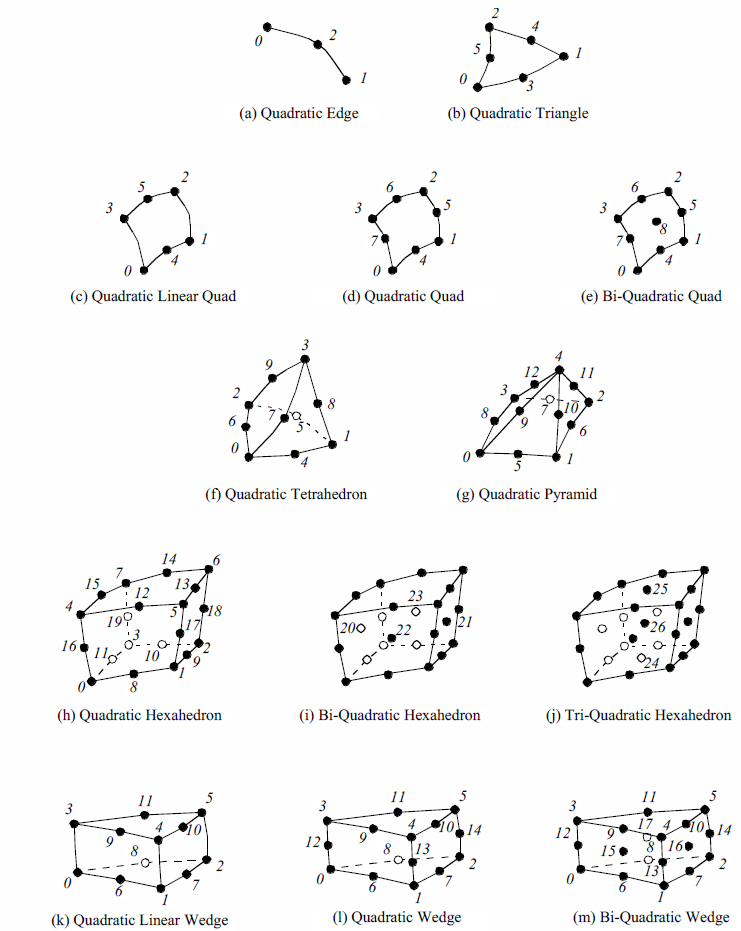
\includegraphics[width=0.8\textwidth]{Figure5-4}
	\caption{Nonlinear cell types found in VTK.}
	\label{fig:Figure5-4}
\end{figure}

One significant difference between linear and nonlinear cells is the way they are rendered and operated on by various visualization algorithms. Linear cells are readily converted to linear graphics primitives, which are then processed by the graphics library. Nonlinear cells, on the other hand, do not often have direct support in graphics libraries. (One exception are the family of non--uniform rational B--splines or NURBS. And even these are generally tessellated by the graphics library into linear primitives.) Therefore, nonlinear cells must be treated specially by the visualization system. Some possibilities include:

\begin{enumerate}

\item Tessellating nonlinear cells into linear cells and then operating on the linear cells.

\item Develop custom rendering and visualization algorithms to operate directly on nonlinear cells.

\item Program custom rendering operations in the graphics library.

\end{enumerate}

These issues are active topics in visualization research \cite{Schroeder05}. In VTK, tessellation methods are currently employed since once tessellated, a cell can be processed by existing linear algorithms. The difficulty with solutions 2) and 3) above is that the effort to create new rendering and visualization algorithms is significant, possibly requiring different solutions for each type of nonlinear cell. Furthermore, it is likely that the performance found in dedicated rendering hardware (e.g., processing linear cells) would far outstrip any software rendering solution for higher order cells. The difficulty with 1) above is that the tessellation must be performed carefully or unacceptable error can be introduced into visualization. Or, if the cell is over--tessellated, an excessive number of linear primitives will result. Future research points to developing adaptive methods that tessellate on a selected error metric (please see Chapter 8: \nameref{chap:advanced_data_representation} for more information).

\begin{figure}[!htb]
	\floatbox[{\capbeside\thisfloatsetup{capbesideposition={right,center},capbesidewidth=0.4\textwidth}}]{figure}[\FBwidth]
	{\caption{Decomposing quadratic nonlinear cells into linear cells. The quadratic tetrahedron is tessellated into six linear tetrahedron; the quadratic hexahedron is tessellated into eight linear hexahedra. Note that some tessellations require the addition of new points. In VTK, a cell adaptor framework is available for tessellating cells with basis functions of arbitrary complexity, see Chapter 8: \nameref{chap:advanced_data_representation} for more information.}\label{fig:Figure5-5}}
	{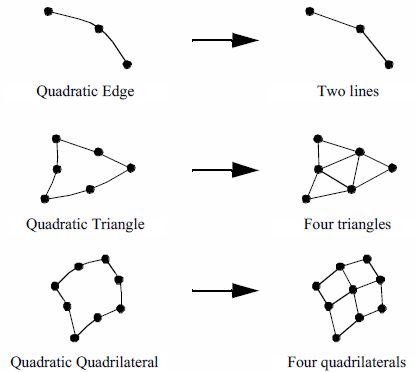
\includegraphics[width=0.6\textwidth]{Figure5-5}}
\end{figure}

VTK tessellates nonlinear quadratic cells using a fixed subdivision as shown in Figure \ref{fig:Figure5-5}. This generally works well for quadratic cells due to the lower order of interpolation, and the few number of points defining the cell.

\begin{description}

\item[Quadratic Edge.\index{cell!quadratic edge}] The quadratic edge is a primary one--dimensional cell. It is defined by three points. The first two points define the endpoints of the edge; the third point is located in the center of the edge as shown in Figure \ref{fig:Figure5-4}. The direction along the line is from the first point to the second point.

\item[Quadratic Triangle.\index{cell!quadratic triangle}] The quadratic triangle is a primary two--dimensional cell. It is defined by six points. The first three points are located at the vertices of the triangle; the next three are located in the middle of each of the three edges as shown in Figure \ref{fig:Figure5-4}.

\item[Quadratic Linear Quadrilateral.\index{cell!quadratic linear quadrilateral}] The quadratic linear quadrilateral is a primary two--dimensional cell. It is defined by six points. The first four points are located at the vertices of the quadrilateral; the next two are located in the middle of each of the first and third edge as shown in Figure \ref{fig:Figure5-4}.

\item[Quadratic Quadrilateral.\index{cell!quadratic quadrilateral}] The quadratic quadrilateral is a primary two--dimensional cell. It is defined by eight points. The first four points are located at the vertices of the quadrilateral; the next four are located in the middle of each of the four edges as shown in Figure \ref{fig:Figure5-4}.

\item[Bi--Quadratic Quadrilateral.\index{bi-quadratic quadrilateral}\index{cell!bi-quadratic quadrilateral}] The bi--quadratic quadrilateral is a primary two-dimensional cell. It is defined by nine points. The first four points are located at the vertices of the quadrilateral; the next four are located in the middle of each of the four edges; and the last one is located at the center of the quadrilateral as shown in Figure \ref{fig:Figure5-4}.

\item[Quadratic Tetrahedron.\index{cell!quadratic tetrahedron}] The quadratic tetrahedron is a primary three--dimensional cell. It is defined by ten points. The first four points are located at the vertices of the tetrahedron; the next six are located in the middle of each of the six edges as shown in Figure \ref{fig:Figure5-4}.

\item[Quadratic Pyramid.\index{cell!quadratic pyramid}] The quadratic pyramid is a primary three--dimensional cell. It is defined by thirteen points. The first five points are located at the vertices of the pyramid; the next eight are located in the middle of each of the eight edges as shown in Figure \ref{fig:Figure5-4}.

\item[Quadratic Linear Wedge.\index{cell!quadratic linear wedge}] The quadratic linear wedge is a primary three--dimensional cell. It is defined by twelve points. The first six points are located at the vertices of the wedge; the next six are located in the middle of each of the six edges that belong to a triangle face as shown in Figure \ref{fig:Figure5-4}.

\item[Quadratic Wedge.\index{cell!quadratic wedge}] The quadratic wedge is a primary three--dimensional cell. It is defined by fifteen points. The first six points are located at the vertices of the wedge; the next nine are located in the middle of each of the nine edges as shown in Figure \ref{fig:Figure5-4}.

\item[Bi--Quadratic Wedge.\index{bi-quadratic wedge}\index{cell!bi-quadratic wedge}] The bi--quadratic wedge is a primary three--dimensional cell. It is defined by eighteen points. The first six points are located at the vertices of the wedge; the next nine are located in the middle of each of the nine edges; and the next three are located in the center of each quadrilateral faces as shown in Figure \ref{fig:Figure5-4}.

\item[Quadratic Hexahedron.\index{cell!quadratic hexahedron}] The quadratic hexahedron is a primary three--dimensional cell. It is defined by twenty points. The first eight points are located at the vertices of the hexahedron; the next twelve are located in the middle of each of the twelve edges as shown in Figure \ref{fig:Figure5-4}.

\item[Bi--Quadratic Hexahedron.\index{bi-quadratic hexahedron}\index{cell!bi-quadratic hexahedron}] The bi--quadratic hexahedron is a primary three--dimensional cell. It is defined by twenty--four points. The first eight points are located at the vertices of the hexahedron; the next twelve are located in the middle of each of the twelve edges; and the next four points are located in the center of the first four faces as shown in Figure \ref{fig:Figure5-4}.

\item[Tri--Quadratic Hexahedron.\index{cell!tri--quadratic hexahedron}] The tri--quadratic hexahedron is a primary three--dimensional cell. It is defined by twenty--seven points. The first eight points are located at the vertices of the hexahedron; the next twelve are located in the middle of each of the twelves edges; the next six are located in the center of each faces; and the last one is located in the center of the hexahedron as shown in Figure \ref{fig:Figure5-4}.
\index{cell|)}

\section{Attribute Data}
\index{cell!attribute|(}
\index{dataset!attributes|(}\index{dataset attributes|(}

Attribute data is information associated with the structure of the dataset. This structure includes both the dataset geometry and topology. Most often, attribute data is associated with dataset points or cells, but sometimes attribute data may be assigned to cell components such as edges or faces. Attribute data may also be assigned across the entire dataset, or across a group of cells or points. We refer to this information as attribute data because it is an attribute to the structure of the dataset. Typical examples include temperature or velocity at a point, mass of a cell, or heat flux into and out of a cell face.

\end{description}
\begin{figure}[!htb]
	\centering
	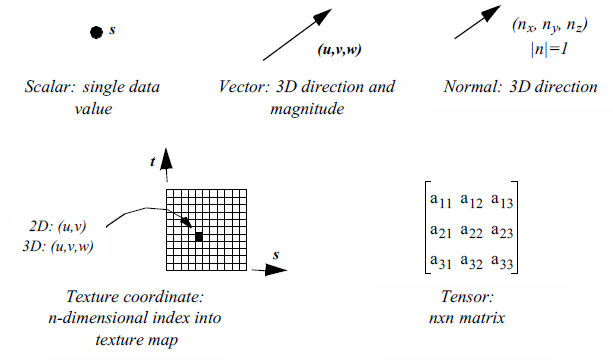
\includegraphics[width=0.8\textwidth]{Figure5-6}
	\caption{Attribute data.}
	\label{fig:Figure5-6}
\end{figure}

Attribute data is often categorized into specific types of data. These categories have been created in response to common data forms. Visualization algorithms are also categorized according to the type of data they operate on.

Single--valued functions, such as temperature or pressure, are examples of scalar data, which is one attribute type. More generally, attribute data can be treated as n-dimensional data arrays. For example, the single-valued function temperature can be treated as a $1 \times 1$ array, while velocity can be treated as a $3 \times 1$ array of components in the x, y, and z directions. This abstract model for data attribute can be extended throughout the visualization system. Some systems extend this model to include the structure of the data. For example, a 3D image dataset (i.e., a volume) can be represented as a 3D array of $l \times m \times n$ data values. Unstructured data can be represented as a 3D vector of position, plus an array of connectivity. We refer to this general approach as the hyperdata model for visualization data (see ``Other Data Abstractions'' on page \pageref{sec:other_data_abstractions}).

In the following sections we describe data attributes using the simpler type--specific model (Figure \ref{fig:Figure5-6}). We also limit ourselves to three-dimensional structure, since the dataset structure and graphics are assumed to be three-dimensional.

\begin{description}

\item[Scalars.\index{dataset attributes!scalars}] Scalar data is data that is single valued at each location in a dataset. Examples of scalar data are temperature, pressure, density, elevation, and stock price. Scalar data is the simplest and most common form of visualization data.

\item[Vectors.\index{dataset attributes!vectors}] Vector data is data with a magnitude and direction. In three dimensions this is represented as a triplet of values $(u, v, w)$. Examples of vector data include flow velocity, particle trajectory, wind motion, and gradient function.

\item[Normals.\index{dataset attributes!normals}] Normals are direction vectors: that is, they are vectors of magnitude $|n|=1$. Normals are often used by the graphics system to control the shading of objects. Normals also may be used by some algorithms to control the orientation or generation of cell primitives, such as creating ribbons from oriented lines.

\item[Texture Coordinates.\index{dataset attributes!texture coordinates}] Texture coordinates are used to map a point from Cartesian space into a $1-$, $2-$, or $3-$dimensional texture space. The texture space is usually referred to as a texture map. Texture maps are regular arrays of color, intensity, and/or transparency values that provide extra detail to rendered objects.

One application of texturing in two dimensions is to ``paste'' a photograph onto one or more polygons, yielding a detailed image without a large number of graphics primitives. (Texture mapping is covered in more detail in Chapter 7:  \nameref{chap:advanced_computer_graphics}.)

\item[Tensors.\index{dataset attributes!tensors}] Tensors are complex mathematical generalizations of vectors and matrices. A tensor of rank k can be considered a k--dimensional table. A tensor of rank $0$ is a scalar, rank $1$ is a vector, rank $2$ is a matrix, and a tensor of rank $3$ is a three-dimensional rectangular array. Tensors of higher rank are k--dimensional rectangular arrays.

General tensor visualization is an area of current research. Efforts thus far have been focused on two--dimensional, rank 2 tensors, which are $3 \times 3$ matrices. The most common form of such tensors are the stress and strain tensors, which represent the stress and strain at a point in an object under load. VTK only treats real-valued, symmetric $3 \times 3$ tensors.

\end{description}
\index{cell!attribute|)}
\index{dataset!attributes|)}\index{dataset attributes|)}

\section{Types of Datasets}
\label{sec:types_of_datasets}
\index{dataset!types|(}\index{dataset types|(}

A dataset consists of an organizing structure plus associated attribute data. The structure has both topological and geometric properties and is composed of one or more points and cells. The type of a dataset is derived from the organizing structure, and specifies the relationship that the cells and points have with one another. Common dataset types are shown in Figure \ref{fig:Figure5-7}.

\begin{figure}[!htb]
	\centering
	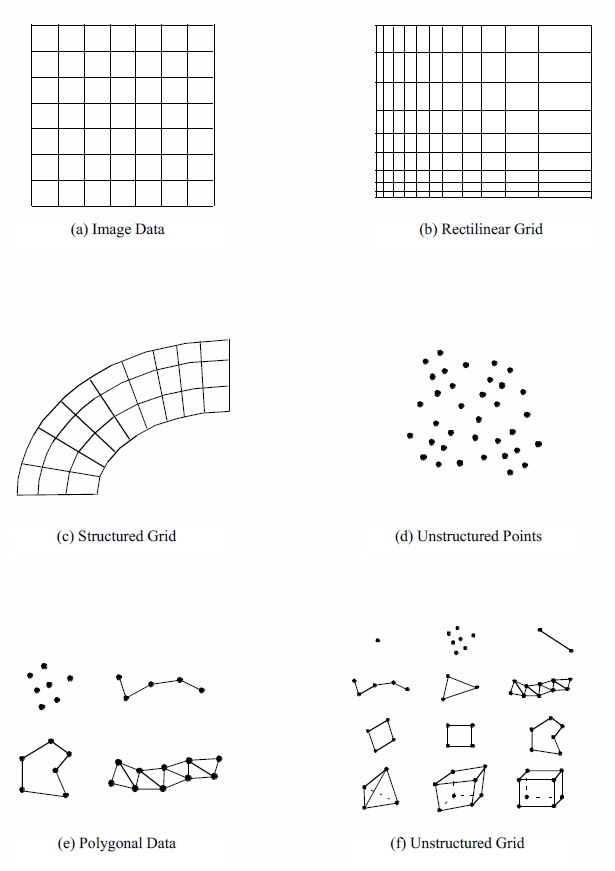
\includegraphics[width=0.8\textwidth]{Figure5-7}
	\caption{Dataset types. The unstructured grid consists of all cell types.}
	\label{fig:Figure5-7}
\end{figure}

A dataset is characterized according to whether its structure is regular or irregular. A dataset is regular if there is a single mathematical relationship within the composing points and cells. If the points are regular, then the geometry of the dataset is regular. If the topological relationship of cells is regular, then the topology of the dataset is regular. Regular (or structured) data can be implicitly represented, at great savings in memory and computation. Irregular (or unstructured) data must be explicitly represented, since there is no inherent pattern that can be compactly described. Unstructured data tends to be more general, but requires greater memory and computational resources.

\subsection{Polygonal Data}
\index{dataset types!polygonal|(}

We have already seen how graphics libraries are designed to render such geometric primitives as lines and polygons. These primitives also are frequently generated or consumed by computational geometry and visualization algorithms. In the Visualization Toolkit, we call this collection of graphics primitives polygonal data. The polygonal dataset consists of vertices, polyvertices, lines, polylines, polygons, and triangle strips. The topology and geometry of polygonal data is unstructured, and the cells that compose that dataset vary in topological dimension. The polygonal dataset forms a bridge between data, algorithms, and high--speed computer graphics.

Vertices, lines, and polygons form a minimal set of primitives to represent 0--, 1--, and 2--dimensional geometry. We have included polyvertex, polyline, and triangle strip cells for convenience, compactness, and performance. Triangle strips in particular are high-performing primitives. To represent n triangles with a triangle strip requires just n+2 points, compared to the 3n points for conventional representations. In addition, many graphics libraries can render triangle strips at higher speeds than triangle polygons.

Our minimal selection of cells is based on common application and performance, representing a subset of the cells available in some graphics libraries. Other types include quadrilateral meshes, Bezier curves and surfaces, and other spline types such as NURBS (Non--Uniform Rational B--Splines) \cite{Mortenson85}. Spline surfaces are generally used to accurately model and visualize geometry. Few visualization algorithms (other than geometry visualization) have been developed that require spline surfaces.
\index{dataset types!polygonal|)}

\subsection{Image Data}
\label{subsec:image_data}
\index{dataset types!image data|(}

An image dataset is a collection of points and cells arranged on a regular, rectangular lattice. The rows, columns, and planes of the lattice are parallel to the global $x-y-z$ coordinate system. If the points and cells are arranged on a plane (i.e., two-dimensional) the dataset is referred to as a pixmap, bitmap, or image. If the points and cells are arranged as stacked planes (i.e., three-dimensional) the dataset is referred to as a volume. Keep in mind that the term image data refers to images, volumes, or one-dimensional point arrays collectively. Note that some authors have referred to image data as uniform grids and structured points. (Structured points was the terminology used in earlier versions of VTK.)

Image data consist of line elements (1D), pixels (2D), or voxels (3D). Image data is regular in both geometry and topology and can be implicitly represented. The representational scheme requires only data dimensions, an origin point, and the data spacing. The dimension of the data is a 3--vector ($n_x,n_y,n_z)$) , specifying the number of points in the $x$, $y$, and $z$ directions. The origin point is the position in three-dimensional space of the minimum $x-y-z$ point. Each pixel (2D) or voxel (3D) in a image dataset is identical in shape, the spacing specifying the length in the $x-y-z$ directions.

The regular nature of the topology and geometry of the image dataset suggests a natural $i-j-k$ coordinate system. The number of points in the dataset is $n_x \times n_y \times n_z$ while the number of cells is $(n_x – 1) \times (n_y – 1) \times (n_z – 1)$. A particular point or cell can be selected by specifying the three indices $i-j-k$. Similarly, a line is defined by specifying two out of three indices, and a plane by specifying a single index.

The simplicity and compactness of representation are desirable features of image data. It is an efficient structure to traverse and compute with. For this reason image data is rivaled only by polygonal data as the most common form of visualization dataset. The major disadvantage with image data is the so--called ``curse of dimensionality''. To obtain greater data resolution we must increase the dimensions of the dataset. Increasing the dimensions of an image results in an $O(n^2)$ increase in memory requirement, while volumes require an $O(n^3)$ increase. Therefore, to resolve a small feature using image data may require more disk space or computer memory than is available.

Image datasets are often used in imaging and computer graphics. Volumes are frequently generated from medical imaging technologies such as Computed Tomography (CT) and Magnetic Resonance Imaging (MRI). Sometimes volumes are used to sample mathematical functions or numerical solutions.
\index{dataset types!image data|)}

\subsection{Rectilinear Grid}
\index{dataset types!rectilinear grid|(}

The rectilinear grid dataset is a collection of points and cells arranged on a regular lattice. The rows, columns, and planes of the lattice are parallel to the global $x-y-z$ coordinate system. While the topology of the dataset is regular, the geometry is only partially regular. That is, the points are aligned along the coordinate axis, but the spacing between points may vary.

Like the image dataset, rectilinear grids consist of pixels (2D) or voxels (3D). The topology is represented implicitly by specifying grid dimensions. The geometry is represented by maintaining a list of separate x, y, and z coordinates. To obtain the coordinates of a particular point, values from each of the three lists must be appropriately combined.
\index{dataset types!rectilinear grid|)}

\subsection{Structured Grid}
\index{dataset types!structured grid|(}

A structured grid is a dataset with regular topology and irregular geometry. The grid may be warped into any configuration in which the cells do not overlap or self--intersect.

The topology of the structured grid is represented implicitly by specifying a 3--vector of dimensions $(n_x, n_y, n_z)$. The geometry is explicitly represented by maintaining an array of point coordinates. The composing cells of a structured grid are quadrilaterals (2D) or hexahedron (3D). Like image data, the structured grid has a natural coordinate system that allows us to refer to a particular point or cell using topological $i-j-k$ coordinates.

Structured grids are commonly found in finite difference analysis. Finite difference is a numerical analysis technique to approximate the solution to partial differential equations. Typical applications include fluid flow, heat transfer, and combustion.
\index{dataset types!structured grid|)}

\subsection{Unstructured Points}
\index{dataset types!unstructured points|(}

Unstructured points are points irregularly located in space. There is no topology in an unstructured point dataset, and the geometry is completely unstructured. The vertex and polyvertex cells are used to represent unstructured points.

Unstructured points are a simple but important type of dataset. Often data has no inherent structure, and part of the visualization task is to discover or create it. For example, consider a piston in a car instrumented with temperature gauges. The number of gauges and their location is chosen at a finite set of points, resulting in temperature values at ``unrelated'' (at least in terms of visualization topology) positions on the surface of the piston. To visualize the surface temperature, we have to create an interpolation surface and scheme to fill in intermediate values.

Unstructured points serve to represent such unstructured data. Typically, this data form is transformed into another more structured form for the purposes of visualization. Algorithms for transforming unstructured points into other forms are described in ``Visualizing Unstructured Points'' on page \pageref{subsec:visualizing_unstructured_points}.
\index{dataset types!unstructured points|)}

\subsection{Unstructured Grid}
\index{dataset types!unstructured grid|(}

The most general form of dataset is the unstructured grid. Both the topology and geometry are completely unstructured. Any cell type can be combined in arbitrary combinations in an unstructured grid. Hence the topology of the cells ranges from 0D (vertex, polyvertex) to 3D (tetrahedron, hexahedron, voxel). In the Visualization Toolkit any dataset type can be expressed as an unstructured grid. We typically use unstructured grids to represent data only when absolutely necessary, because this dataset type requires the most memory and computational resources to represent and operate on.
\index{dataset types!unstructured grid|)}

\index{dataset!types|)}\index{dataset types|)}

\section{Other Data Abstractions}
\label{sec:other_data_abstractions}

Other data models have been proposed besides the dataset model presented here. We briefly examine two other models that have been applied successfully. These are the AVS field model and the model of Haber, Lucas, and Collins, adapted in modified form by the commercial IBM Data Explorer\index{Data Explorer} system. The section concludes with a brief comparison between these two models and VTK's data model.

\subsection{The Application Visualization System}

AVS (the Application Visualization System)\index{Application Visualization System|see {AVS}}\index{AVS} was the first large--scale, commercial visualization system \cite{AVS89}. Much of the early growth, visibility, and successful application of visualization technology was achieved because of the direct application of AVS or the influence of AVS on other researchers. AVS is a data-flow visualization system with a crisp user interface to create, edit, and manipulate visualization networks. Using an explicit executive to control execution of networks, AVS can run distributed and parallel visualization applications. Since the AVS architecture is open, researchers and developers can and have donated filters for use by others.

The AVS data model consists of primitive data and aggregate data. Primitive data are fundamental representations of data such as byte, integer, real, and string. Aggregate types are complex organizations of primitive types and include fields, colormaps, geometries, and pixel maps. Fields can be considered AVS's fundamental data type, and will be described in detail shortly. Colormaps are used to map functional values (i.e., scalar values) into color and transparency values. Geometries consist of graphics primitives such as points, lines, and polygons, and are used by the geometric renderer to display objects. A pixel map is the rendered image, or output, of a visualization.

The field is the most interesting part of the AVS data model. In general, it is an n--dimensional array with scalar or vector data at each point. A scalar is a single value, while a vector is two or more values (not necessarily three). The field array can have any number of dimensions, and the dimensions can be of any size. There is no implicit structure to the field, instead, a mapping function is defined. That is, either an implicit or explicit relationship from data elements to coordinate points is specified. Thus a field is a mapping between two kinds of space: the computational space of the field data and the coordinate space, which is typically the global coordinate system. AVS supports three types of mappings: uniform (i.e., structured), rectilinear, and irregular (i.e., unstructured).

\subsection{The Data Explorer}

The data model of Haber, Lucas, and Collins \cite{Haber91} is based on the mathematics of fiber bundles. The goal of their work is to create a general model for piecewise representations of fields on regular and irregular grids. They refer to their model as the field data model, but their definition of the word field is different from the AVS model. A field is an object composed of a base and dependent data. Informally, the base is a manifold whose coordinates are the independent variables for the field, and the dependent data relate the values of dependent variables to the independent variables of the base. Visualization data consists of field elements that describe the base and dependent variables over a local region.

\subsection{The Visualization Toolkit}
\index{Data Explorer!and VTK|(}

There are similarities and differences between these data models and VTK's dataset model. The greatest difference is that these other models are more abstract. They are capable of representing a wider range of data and are more flexible. In particular, the AVS\index{AVS!and VTK} field model is capable of representing arbitrary streams of numbers in a simple and elegant manner. The field data model of Haber et al. is also powerful: The authors show how this data representation can be used to exploit regularity in data to obtain compact representations. On the other hand, all these models (including VTK's) share the notion of structure versus data. The AVS field model introduces structure by using a mapping function. The field data of the Haber et al. model resembles VTK's dataset model, in that the base is equivalent to VTK's cells, and the field data model's dependent data is analogous to VTK's attribute data.

The difference in abstraction level raises important issues in the design of visualization systems. In the following discussion we refer to data models as abstract or concrete, where the relative level of abstraction is lower in concrete models. Abstract and concrete classes compare as follows:

\begin{itemize}

	\item Abstract models are more flexible and capable of representing a wider range of data forms than concrete models.

	\item Abstract models lend themselves to compact computer code.

	\item Concrete models are easier to describe, interface, and implement than abstract models.

	\item The level of abstraction influences the computer code and/or database interface to the data model. Abstract models result in abstract code and data representations; concrete models result in concrete code and data representations.

	\item The complexity of abstract models can be hidden by creating simpler, application--specific interfaces. However, this requires extra effort. Concrete models, on the other hand, cannot be made more abstract by modifying interfaces.

\end{itemize}

The design of computer systems demands careful attention to the balance between abstract and concrete systems. Visualization systems, in particular, must be carefully designed because they interface to other systems and data models. Models that are too abstract can result in confusing computer code and interfaces, and can be misused because of user misunderstanding. On the other hand, concrete models are limited in flexibility and capability, but tend to be easier to learn and apply.

In the design of the Visualization Toolkit, we chose to use a more concrete data model relative to the AVS and field data models. Our decision was based on the premise that the system was to be informative as well as functional, and we wanted to clearly demonstrate basic concepts. On the other hand, VTK's data model is general enough to support our practice of visualization. Our experience with users also has shown us that VTK's data model is easier for the casual visualization user to understand than the more abstract models. If you decide to design your own system, we recommend that you examine other data models. However, we feel that the clarity of code manifested in the Visualization Toolkit is an example of a well--balanced trade--off between design abstraction and simplicity.
\index{Data Explorer!and VTK|)}

\section{Putting It All Together}

In this section we will describe the implementation details of the dataset types covered previously. We will also show you how to create these datasets through a variety of C++ examples.

\subsection{Memory Allocation and Data Arrays}

Because of the size and scope of data, memory must be carefully managed to create efficient visualization systems. In the Visualization Toolkit, we use contiguous data arrays as the basis for most data structures. Contiguous arrays can be created, deleted, and traversed faster than alternative data structures, such as linked lists or arrays of pointers to structures. In VTK, we refer to these as data arrays\index{data array}, and represent them with the class vtkDataArray.

Contiguous arrays also can be easily transmitted across a network, particularly if the information in the array is independent of computer memory address. Memory independence avoids the overhead of mapping information from one memory location to another. Therefore, in VTK we access information based on an ``id'', an integer index into an array--like object. Data arrays are 0 offset just like C++ arrays. That is, given n data values, we successively access these values using the ids $(0, 1, 2, ..., n – 1)$.

An important design decision was to not represent data using arrays of objects (e.g., a separate class for cells and/or points). Our experience has shown that such designs severely impact performance due to the cost of construction and deletion. Instead, we focus on designing classes at a higher level of abstraction. From the perspective of performance, the object--oriented approach serves best at the application level, not at the level of implementation.

\begin{figure}[!htb]
	\centering
	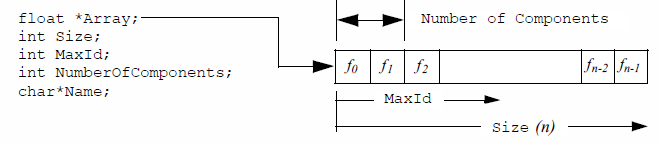
\includegraphics[width=0.8\textwidth]{Figure5-8}
	\caption{Implementation of contiguous array. This example is a fragment of the class definition vtkFloatArray.}
	\label{fig:Figure5-8}
\end{figure}

The class vtkFloatArray is an example of a contiguous array. We will use this class to describe how contiguous arrays are implemented in VTK. As shown in Figure \ref{fig:Figure5-8}, the instance variable Array is a pointer to memory of type float. The allocated length of the array is given by Size. The array is dynamic, so an attempt to insert data beyond the allocated size automatically generates a Resize() operation. When resized, the array approximately doubles in size each time. The MaxId field is an integer offset defining the end of inserted data. If no data has been inserted, then MaxId is equal to -1. Otherwise, MaxId is an integer value where $0 \leq MaxId < Size$.

\subsection{The Tuple Abstraction}

Many visualization data are defined by multiple component values. An x-y-z coordinate triplet or RGBA color pixel value are two such examples. To represent such data in a contiguous data array, the tuple data abstraction is introduced. As Figure \ref{fig:Figure5-8} illustrates, the contiguous array is grouped into smaller subarrays with NumberOfComponents components. These subarrays are called tuples, and for a given array the tuple size, or NumberOfComponents, is constant for all tuples as shown in Figure \ref{fig:Figure5-9}.

\begin{figure}[!htb]
	\centering
	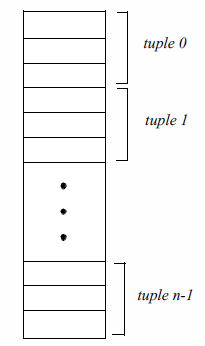
\includegraphics[width=0.3\textwidth]{Figure5-9}
	\caption{Data array structure. In this example, each tuple has 3 components.}
	\label{fig:Figure5-9}
\end{figure}

\subsection{Representing Data With Data Arrays}
\index{data arrays!implementation|(}

Attribute data and points, as well as several other data objects, are represented with data arrays in VTK. Certain attribute data, such as points, vectors, normals, and tensors, are required to have a tuple size consistent with their definition. For example, points, vectors and normals require a data array with a tuple size of three; tensors a tuple size of nine (i.e., a $3 \times 3$ matrix). Scalars do not place any requirement on the tuple size. Algorithms that process such scalar data generally operate on the first component of each tuple. (Filters exist in VTK to split multi-component data arrays into separate arrays, and to combine separate data arrays into a single array. See vtkSplitField and vtkMergeFields).
\index{data arrays!implementation|)}

\subsection{Abstract/Concrete Data Array Objects}

Visualization data comes in many forms --- floating point, integer, byte, and double precision --- to name just a few simple types. More complex types such as character strings or multidimensional identifiers also are possible. Given this variety of types, how do we represent and manipulate such data using data arrays? The answer is to provide run-time solutions via abstract data objects, and compile-time solutions using templated C++ code.

Abstract data objects are objects that provide uniform methods to create, manipulate, and delete data using dynamic binding. In C++ we use the virtual keyword to declare methods as dynamically bound. Dynamic binding allows us to execute a method belonging to a concrete object by manipulating that object's abstract superclass (see Figure \ref{fig:Figure5-10}).

\begin{figure}[!htb]
	\centering
	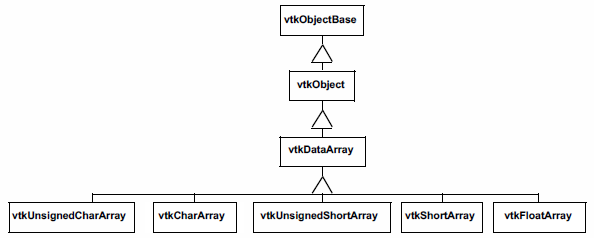
\includegraphics[width=0.8\textwidth]{Figure5-10}
	\caption{Data array object diagram. vtkDataArray is an abstract base class. Subclasses of vtkDataArray implement type specific representation and operations. Note: not all concrete data array subclasses are shown in this diagram.}
	\label{fig:Figure5-10}
\end{figure}

Consider the abstract class vtkDataArray. We can access the data value at associated point id 129 by executing the method \texttt{double s = GetTuple1(129)}. Since the virtual GetTuple1() method returns a floating-point data value, each subclass of vtkDataArray must also return a floating-point value. Although the subclass is free to represent data in any possible form, it must transform its data representation into a floating-point value. This process may be as simple as a cast from a built-in type to floating-point value, or it may be a complex mapping of data. For example, if our data consists of character strings, we could conceivably create an alphabetical list and map the string into a location in the list, and then cast the location into a double value.

While this run-time oriented interface is convenient for writing general algorithms that do not depend on a particular data type, the conversion of native representation to double type is problematic. First, the conversion operation can affect performance adversely, since the data access methods are called frequently, virtual functions are slower than in-line or non-virtual invocations, and the cast operator is slow in many cases. Second, a complex type such as double loses precision during conversion to double. To remedy these problems, it is possible to access data in its native form and process it accordingly. In this approach C++ templates\index{C++!templates} are used.

To use templates it is necessary to obtain raw, typed pointers to data, and to know the type of data. vtkDataArray and its associated subclasses provides this functionality. With this information it is possible to switch on the type of data into a function templated over that type. A typical code fragment using this functionality is found in most imaging filters, almost all of which are templated as follows:

\begin{lstlisting}[language=TCL, caption={Obtaining raw typed pointers to data.}]
switch (outData->GetScalarType())
  {
  case VTK_CHAR:
  { typedef char VTK_TT;
    func(arg1, arg2, arg3, VTK_TT* arg4, VTK_TT* arg5); }
    break;
  case VTK_UNSIGNED_CHAR:
  { typedef unsigned char VTK_TT;
    func(arg1, arg2, arg3, VTK_TT* arg4, VTK_TT* arg5); }
    break;

...for all types.....

\end{lstlisting}

\begin{figure}[!htb]
	\centering
	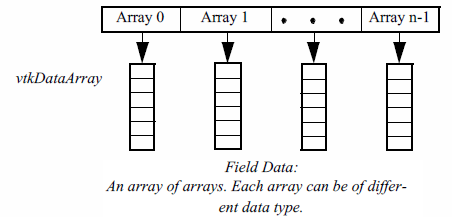
\includegraphics[width=0.8\textwidth]{Figure5-11}
	\caption{Data object representation as field data. A field can be represented as an array of arrays. Each array has a specified type, length, tuple size, and name. The association of a data array with points or cells, and its labeling as a particular attribute type, forms point and cell attribute data.}
	\label{fig:Figure5-11}
\end{figure}

In practice this code is simplified using macros, and the \texttt{static\_cast<>} C++ operator is used to perform the cast. Note that the function func is a templated function. The compiler will instantiate the function for the appropriate type. In most cases all native types are represented in the switch statement, so func is expanded accordingly.

Using compile-time oriented methods such as templates avoids the need to cast each data access into a particular type (e.g., double). While it does complicate the code somewhat and result in larger object code, it is generally faster than run-time virtual methods. This approach becomes problematic as the number of types increases. For example, some filters such as vtkImageShiftScale use doubly nested templates to resolve the potential difference in input and output types. The code is more complex and much larger than the generic run-time approach.

\subsection{Data Object Representation}

Data objects are implemented in VTK as an array of vtkDataArrays as shown in Figure \ref{fig:Figure5-11}. vtkDataObject is an general representation of visualization data. It serves to encapsulate instance variables and methods for visualization network execution (see previous chapter), as well as representing data. Internally, data is represented with an instance of the class vtkFieldData. Very few algorithms directly operate on data objects; rather most algorithms require the specification of an organizing structure in order to process the data. The dataset specifies that organizing structure as described in the following section.

\subsection{Dataset Representation}
\index{dataset!representation|(}\index{dataset representation!implementation|(}

Five datasets are implemented in VTK: vtkPolyData, vtkImageData, vtkStructuredGrid, vtkRectilinearGrid, and vtkUnstructuredGrid. The unstructured points dataset is not implemented, but can be represented using either vtkPolyData or vtkUnstructuredGrid.

We use a different internal data representation for each dataset type. By using different representations we minimize data structure memory requirements and implement efficient access methods. It would have been possible to use vtkUnstructuredGrid to represent all dataset types, but the memory and computational overhead are unacceptable for large data. The following sections describe how we represent the dataset.

\begin{description}

\item[vtkImageData.] The simplest and most compact representation is vtkImageData. Both the dataset points and cells are represented implicitly by specifying the dimensions, data spacing, and origin. The dimensions define the topology of the dataset, while the origin and spacing specify the geometry. The vtkImageData dataset type can represent 1D line samples, 2D images, and 3D volumes. (Note: in earlier versions of VTK, vtkImageData was known as vtkStructuredPoints. There are still remnants of this terminology in the code base.)

There is an implicit ordering of both the points and cells composing vtkImageData. Both the cells and points are numbered in the direction of increasing x, then y, then z. The total number of points is $n_x \times n_y \times n_z$ where $n_x$, $n_y$, and $n_z$z are the dimensions of vtkImageData. The total number of cells is $(n_x - 1) \times  (n_y - 1) \times (n_z - 1)$.

\item[vtkRectilinearGrid.] While the topology of vtkRectilinearGrid is regular, the geometry can be described as ``semi-regular''. The topology is implicitly represented by specifying data dimensions along the x, y, and z coordinate axes. The geometry is defined using three arrays of coordinate values along these axes. These three coordinate arrays can be combined to determine the coordinates of any point in the dataset. In VTK, we represent the arrays using three instances of vtkDataArray. The numbering of points and cells is implicit in exactly the same way as described for vtkImageData.

\item[vtkStructuredGrid.] Like vtkImageData, the topology of vtkStructuredGrid is regular and is defined by specifying dimensions in the topological $i-j-k$ coordinate system. However, the geometry of vtkStructuredGrid is realized by specifying point coordinates in the global $x-y-z$ coordinate system.

The abstract data class vtkPoints is used to represent the point coordinates. vtkPoints refers to an underlying instance of vtkDataArray which actually holds the representation of the points as a contiguous array of three-component tuples. A particular point coordinate may be retrieved or inserted by specifying a particular point id. The numbering of the points and cells is implicit in the same fashion as vtkImageData. Care must be taken to insure that the number of points in the data array is the same as that implied by the dimensions of the grid.

\item[vtkPolyData.] Unlike vtkImageData and vtkStructuredGrid, the topology of vtkPolyData is not regular, so both the topology and geometry of the dataset must be explicitly represented. The point data in vtkPolyData is represented using the vtkPoints class similar to vtkStructuredGrid.

\begin{figure}[!htb]
	\centering
	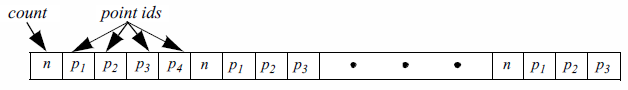
\includegraphics[width=0.8\textwidth]{Figure5-12}
	\caption{vtkCellArray structure to represent cell topology.}
	\label{fig:Figure5-12}
\end{figure}

The Visualization Toolkit uses the class vtkCellArray to explicitly represent cell topology. This class is a list of connectivity for each cell. The structure of the list is a sequence of integer numbers (Figure \ref{fig:Figure5-12}). The first number in the list is a count (the number of points in the cell connectivity), and the next series of numbers is the cell connectivity. (Each number in the connectivity list is an index into an instance of a point coordinate list.) Sequences of count followed by the connectivity list are repeated until each cell is enumerated. Additional information such as the number of cells in the list and current position in the list (for traversal purposes) is also maintained by vtkCellArray.

Notice that type information is not directly represented in this structure. Instead, vtkPolyData maintains four separate lists to vertices, lines, polygons, and triangle strips. The vertex list represents cells of type vtkVertex and vtkPolyVertex. The lines list represents cells of type vtkLine and vtkPolyLine. The polygon list represents cells of type vtkTriangle, vtkQuad, and vtkPolygon. The triangle strip list represents cells of the single type vtkTriangleStrip. As a result, the cell type is known from the particular list the cell is defined in, plus the number of points that define the cell.

Our design of the vtkPolyData class is based on two important requirements. First, we want an efficient interface to external graphics libraries. Second, we wish to aggregate cells according to topology. The four separate lists provide efficient interface because graphics libraries have separate vertex, line, polygon, and triangle strip primitives. As a result, in VTK no run-time checking is required to match the different cell types with the appropriate ``load primitive'' function, since the type is known from the list in which the primitive resides. The four lists also separate cells into 0-, 1-, and 2-dimensional types. This is useful because visualization algorithms often treat data of varying topological order differently.

\item[vtkUnstructuredGrid.] The dataset type vtkUnstructuredGrid is the most general in terms of its ability to represent topological and geometric structure. Both points and cells are explicitly represented using derived classes of vtkPoints and vtkCellArray. The class vtkUnstructuredGrid is similar to vtkPolyData except that vtkUnstructuredGrid must be capable of representing all cell types, not just the limited graphics types (i.e., vertices, lines, polygons, and triangle strips) of vtkPolyData.

Another distinguishing characteristic of vtkUnstructuredGrid is that we represent type information differently. In vtkPolyData we categorized cells into four separate lists, thereby representing cell type indirectly. In vtkUnstructuredGrid we add the additional class vtkCellTypes to represent cell type explicitly.

The vtkCellTypes is an array of supplemental information. For each cell, an integer flag defines the cell type. Another variable is used to record the location of the cell definition in the corresponding vtkCellArray (Figure \ref{fig:Figure5-13}).

Besides representing cell type, this design also enables random access to cells. Because the length of a cell connectivity list varies, the vtkCellArray class cannot locate a particular cell without traversing its data structure from the origin. With the added class vtkCellTypes, however, it is possible to directly access a cell with a single dereference (i.e., using the offset value).

The vtkCellTypes may also be added to the vtkPolyData data representation  --- and indeed it has. However, our reasons for this addition are not to represent type explicitly, but rather to provide random access to the cells and enable many topological operations. We will expand on this idea in Chapter 8: \nameref{chap:advanced_data_representation}.

\item[Object Model.] The five datasets are implemented as shown in Figure \ref{fig:Figure5-14}. As this object diagram illustrates, these concrete datasets are subclasses of the abstract class vtkDataSet. Two additional classes are introduced as well. The class vtkStructuredData contributes instance variables and methods for structured data. vtkStructuredData is not in an inheritance relationship with the datasets; rather the structured datasets shown delegate to it in order to implement some of their methods. (This was done to avoid multiple inheritance.) Subclasses of the class vtkPointSet represent their points explicitly, that is, through an instance of vtkPoints or its subclasses. vtkPointSet provides methods and instance variables to manipulate the point data, as well as a general searching capability to find points and cells. (See ``Searching'' on page \pageref{sec:searching} for more information.)

\end{description}


\begin{figure}[!htb]
	\floatbox[{\capbeside\thisfloatsetup{capbesideposition={right,center},capbesidewidth=0.3\textwidth}}]{figure}[\FBwidth]
	{\caption{The data structure of the class vtkUnstructuredGrid. (This is a subset of the complete structure. See Chapter 8: \nameref{chap:advanced_data_representation} for complete details.}\label{fig:Figure5-13}}
	{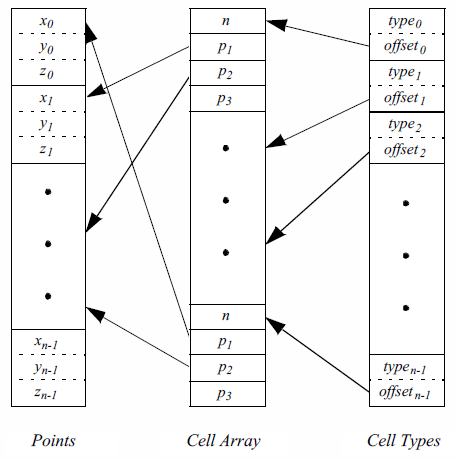
\includegraphics[width=0.6\textwidth]{Figure5-13}}
\end{figure}



\begin{figure}[!htb]
	\centering
	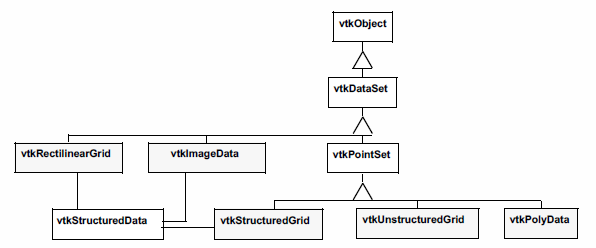
\includegraphics[width=0.8\textwidth]{Figure5-14}
	\caption{Dataset object diagram. The five datasets (shaded) are implemented in VTK.}
	\label{fig:Figure5-14}
\end{figure}

\begin{figure}[!htb]
	\centering
	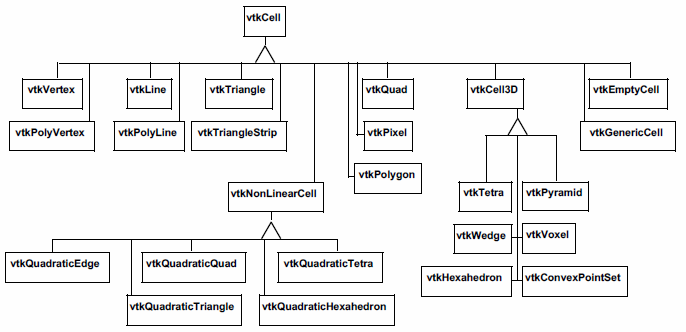
\includegraphics[width=0.8\textwidth]{Figure5-15}
	\caption{Object diagram for twenty concrete cell types in VTK. vtkEmptyCell represents NULL cells. vtkGenericCell can represent any type of cell. Three-dimensional cells are subclasses of vtkCell3D. Higher order cells are subclasses of vtkNonLinearCell.}
	\label{fig:Figure5-15}
\end{figure}

\index{dataset!representation|)}\index{dataset representation!implementation|)}

\subsection{Cell Representation}
\index{cell!representation!implementation|(}

In the \emph{Visualization Toolkit} each cell type has been implemented by creating specific classes. Each cell is a subclass of the abstract type vtkCell . Cell topology is represented by a list of ordered point ids, and cell geometry is represented by a list of point coordinates. The object diagram for vtkCell and its subclasses is shown in Figure \ref{fig:Figure5-15}.

The abstract class vtkCell specifies methods that each cell must implement. These methods provide a defined interface to the cell's geometry and topology. Additional methods perform computation on the cell. These methods will be discussed in detail in Chapter 8: \nameref{chap:advanced_data_representation}.
\index{cell!representation!implementation|)}

\subsection{Data Attributes}
\index{dataset attributes!implementation|(}

Data attributes are associated with the structure of a dataset. The dataset model is built on points and cells, so it is natural to associate data attributes with points and cells as well. Intermediate structure features, such as cell edges or faces, are not explicitly represented so we cannot easily associate data attributes with them.

In VTK data attributes are associated with the points and cells of the dataset. There is no association of data attributes to intermediate topological features such as triangle edges or hexahedron faces. (Here we refer to data attributes associated with points as point attributes, and data attributes associated with cells as \emph{cell attributes}\index{cell attributes}.) Our design choice is based on the following rationale.

\begin{itemize}

	\item Data acquisition and numerical simulation systems typically measure and/or compute the results at point locations, or at the center of cells.

	\item Boundary attribute information (e.g., on faces and edges) can be maintained as cell data ordered according to the topology of the cell.

	\item The VTK data model is based on points and cells for reasons of compactness and efficiency. Representing attribute data on cell boundaries would require expanding this representation to support a small number of situations requiring direct support of attribute data on cell boundaries. If in the future a more complex data structure is required to represent boundary attribute data, this is best encapsulated into a single class rather than forcing the abstraction throughout the system.

\end{itemize}
\begin{figure}[!htb]
	\centering
	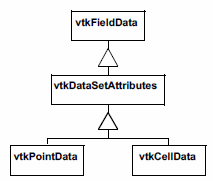
\includegraphics[width=0.8\textwidth]{Figure5-16}
	\caption{Inheritance hierachy for representing data set attributes.}
	\label{fig:Figure5-16}
\end{figure}

One difficulty with maintaining both cell data and point data representations is that possible inconsistencies in the data may arise. For example, if a cell's scalar value is 0.5, and its points have scalar values other than 0.5, which is the correct value? Priority schemes can be devised to resolve such situations although the user must recognize that such inconsistencies may exist.

To represent dataset attributes we use the organizing classes vtkPointData and vtkCellData, both of which are subclasses of the class vtkFieldData as shown in Figure \ref{fig:Figure5-1}. The class vtkDataSetAttributes serves to coordinate the movement of datafrom one process object to the next. It provides methods for copying, interpolating, and moving data between input and output.

Another important feature of vtkDataSetAttributes is that it provides the ability to assign a data array to represent a particular data attribute. For example, the method SetScalars() is used to specify which data array is to be treated as the scalars in the field.

There is a one-to-one correspondence between each dataset point and its attribute data. Point attributes are accessed by way of the point id. For example, to access the scalar value of point id 129 in the dataset instance aDataSet, we use a

\begin{lstlisting}[language=C++,  caption={}, numbers=none, frame=none]
\texttt{DataSet->GetPointData()->GetScalars()->GetTuple(129);}
\end{lstlisting}

This statement assumes that the scalar data has been defined for this dataset and is non-NULL.
\index{dataset attributes!implementation|)}

\subsection{Examples}

In the examples that follow we show manual creation and manipulation of datasets. Typically, these operations are not performed directly by users of VTK. Instead, source objects are used to read data files or generate data. This is more convenient than the manual techniques shown here and should be used whenever possible.

Creation of datasets is a two step process. First the geometry and topology of the dataset must be defined. Depending on the type of dataset, the geometry and topology definition will proceed differently. Then the point and/or cell attribute data is created and associated with the dataset. Remember that there is a one-to-one relationship between the attribute data and the points and cells in the dataset.



\subsubsection{Create a Polygonal Dataset}

In our first example we create a polygonal representation of a cube. The cube is defined by eight points and six quadrilateral faces. We also create eight scalar values associated with the eight vertices of the cube. Figure \ref{fig:Figure5-17} shows the key C++ code fragments used to create the data, and the resulting image.

The geometry of the cube is defined using an instance of the class vtkPoints. By default, the underlying type of vtkPoints is a vtkFloatArray. The topology of the cube (i.e., polygons) is defined with an instance of the class vtkCellArray. These define the points and polygons of the cube, respectively. Scalar data is represented by an instance of the class vtkIntArray.

\begin{figure}[!htb]
	\begin{subfigure}[h]{0.48\linewidth}
		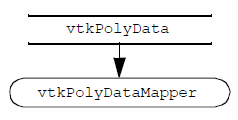
\includegraphics[width=0.96\linewidth]{Figure5-17a}
		\caption*{}
		\label{fig:Figure5-17a}
	\end{subfigure}
	\hfill
	\begin{subfigure}[h]{0.48\linewidth}
		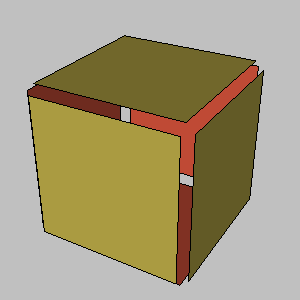
\includegraphics[width=0.96\linewidth]{Figure5-17b}
		\caption*{(\href{https://lorensen.github.io/VTKExamples/site/Cxx/GeometricObjects/Cube/}{Cube.cxx} or \href{https://lorensen.github.io/VTKExamples/site/Python/GeometricObjects/Cube/}{Cube.py})}
		\label{fig:Figure5-17b}
	\end{subfigure}
	\hfill
	\begin{subfigure}[h]{0.96\linewidth}
		\caption*{}
	\end{subfigure}
	\hfill
	\begin{subfigure}[h]{0.96\linewidth}
		\begin{lstlisting}[language=C++, caption={}]
		vtkPolyData *cube = vtkPolyData::New();
		vtkPoints *points = vtkPoints::New();
		vtkCellArray *polys = vtkCellArray::New();
		vtkFloatArray *scalars = vtkFloatArray::New();
		for (i=0; i<8; i++) points->InsertPoint(i,x[i]);
		for (i=0; i<6; i++) polys->InsertNextCell(4,pts[i]);
		for (i=0; i<8; i++) scalars->InsertTuple1(i,i);
		cube->SetPoints(points);
		points->Delete();
		cube->SetPolys(polys);
		polys->Delete();
		cube->GetPointData()->SetScalars(scalars);
		scalars->Delete();
		\end{lstlisting}
		\caption*{}
		\label{fig:Figure5-17c}
	\end{subfigure}
	\caption{Creation of polygonal cube.}\label{fig:Figure5-17}
\end{figure}

As this example shows, polygonal data is created by constructing pieces (e.g., points, cells, and point attribute data), and then assembling the pieces to form the complete dataset. If the name of the instance of vtkPolyData is cube, we can summarize these three steps as follows:

\begin{enumerate}

	\item Create instance of subclass of vtkPoints to define geometry(i.e.,point coordinates). Use the operator cube->SetPoints() to associate the points with the dataset.

	\item Create instances of vtkCellArray to define topology for vertices, lines, polygons, and triangle strips. Use the operators cube->SetVerts(), cube->SetLines(), cube->SetPolys(), and cube->SetStrips() to associate the cells with the dataset.

	\item Create instance of subclass of vtkPoints to define geometry(i.e.,point coordinates). Use the operator cube->SetPoints() to associate the points with the dataset.

	\item Create point and/or attribute data. Every dataset has two fieldsrepresenting vtkPointData and vtkCellData. Use the operator pd=cube->GetPointData() to retrieve the pointer to the point attribute data. Use the operator pd=cube->GetCellData() to retrieve the pointer to the cell attribute data. Associate the attribute data with the dataset using the operators pd->SetScalars(), pd->SetVectors(), pd->SetNormals(), pd->SetTensors(), and pd->SetTCoords() (and similar for cell data).

\end{enumerate}

Polygonal data supports the following cell types: vertices, polyvertices, lines, polylines, triangles, quadrilaterals, polygons, and triangle strips. Point and cell attribute data does not need to be defined  --- you can create none, some, or all of the point and cell attributes in any combination.

The most confusing aspect of this example is the Delete() method. To prevent memory leaks we must use a Delete() method (VTK's destructor) after every New() method. It is apparent from the example that the instance's points, polys, and scalars are referred to by another object (e.g., cube). So doesn’t invocation of the Delete() method pose a problem?

The answer is no. Certain data objects in VTK are reference counted to conserve memory resources (i.e., subclasses of vtkObjectBase). That means they can be shared between objects. For most objects the Delete() will invoke the destructor. Reference counted objects act a little differently. The Delete() method simply decrements the reference count. This may or may not destroy the object depending on whether it is being used by another object. In this example the points, polys, and scalars are used by the polygonal dataset cube, so they are not deleted when Delete() is invoked. They will be freed once we free the dataset cube, that is, when their reference count drops to zero. (See the VTK User's Guide for more information about memory management.)

\subsubsection{Create an Image Data Dataset}

In this example, we create an image dataset (i.e., an instance of vtkImageData). The topology of the dataset is defined by specifying the data dimensions. The geometry is defined by the data spacing and origin. The spacing specifies the length, width, and height of each voxel. The origin specifies the position in 3D space of the ``lower-left'' corner of the data. In our example we set the origin and spacing of the dataset so that its center lies at the origin, and the bounds of the dataset are $(-0.5,0.5, -0.5,0.5, -0.5,0.5)$.

In this example we create scalar data along with the image data dataset. The scalar values are computed from the implicit function for a sphere

\begin{equation}\label{eq:5.2}
F(x,y,z) = (x^2 + y^2 + z^2)-R^2\end{equation}
\myequations{Implicit function for a sphere}

with the radius $R = 0.4$. The scalar data is stored in an instance of vtkFloatArray and assigned to the point attribute data of the dataset.

To complete this example, a contour filter is used to generate a surface of scalar value $F(x, y, z) = 0$. Note that this functionality (in a more general form) is available from the source object vtkSampleFunction in combination with vtkSphere. Figure \ref{fig:Figure5-18} shows the key C++ code fragment used to create the data and contour the scalar field, and the resulting image.

Image data datasets are easy to construct because both the geometry and topology are implicitly defined. If the name of the instance of vtkImageData is vol, we can summarize the steps to create the dataset as follows:

\begin{enumerate}

	\item Define the topology of the dataset using the operator vol->SetDimensions().

	\item Define the geometry of the dataset using the operators vol->SetOrigin() and vol->SetSpacing().

	\item Create point and/or attribute data and associate it with the dataset.

\end{enumerate}

You do not need to specify origin and data spacing. By default the data spacing is $(1,1,1)$ in the $x-y-z$ directions, and the origin is $(0,0,0)$. Thus if the dimensions of the dataset are $(n_x \times n_y \times n_z)$ , the default length, width, and height of the dataset will be $(n_x – 1, n_y – 1, n_z – 1)$.

The topological dimension of the dataset is implicitly known from its instance variables. For example, if any of the dimensions $(n_x, n_y, n_z)$ is equal to one (and the other two are greater than one), the topological dimension of the dataset is two.

\begin{figure}[!htb]
	\begin{subfigure}[h]{0.48\linewidth}
		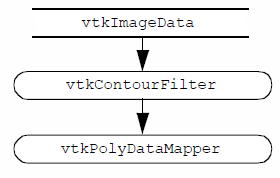
\includegraphics[width=0.96\linewidth]{Figure5-18a}
		\caption*{}
		\label{fig:Figure5-18a}
	\end{subfigure}
	\hfill
	\begin{subfigure}[h]{0.48\linewidth}
		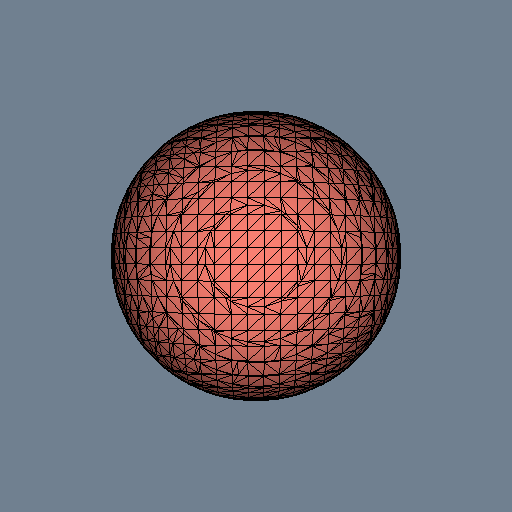
\includegraphics[width=0.96\linewidth]{Figure5-18b}
		\caption*{(\href{https://lorensen.github.io/VTKExamples/site/Cxx/StructuredPoints/Vol/}{Vol.cxx} or \href{https://lorensen.github.io/VTKExamples/site/Python/StructuredPoints/Vol/}{Vol.py})}
		\label{fig:Figure5-18b}
	\end{subfigure}
	\hfill
	\begin{subfigure}[h]{0.96\linewidth}
		\caption*{}
	\end{subfigure}
	\hfill
	\begin{subfigure}[h]{0.96\linewidth}
		\begin{lstlisting}[language=C++, caption={}]
		vtkImageData *vol = vtkImageData::New();
		  vol->SetDimensions(26,26,26);
		  vol->SetOrigin(-0.5,-0.5,-0.5);
		  sp = 1.0/25.0;
		  vol->SetSpacing(sp, sp, sp);

		vtkFloatArray *scalars = vtkFloatArray::New()
		for (k=0; k<26; k++)
		  {
		  z = -0.5 + k*sp;
		  kOffset = k * 26 * 26;
		  for (j=0; j<26; j++)
		    {
		    y = -0.5 + j*sp;
		    jOffset = j * 26;
		    for (i=0; i<26; i++)
		      {
		      x = -0.5 + i*sp;
		      s = x*x + y*y + z*z - (0.4*0.4);
		      offset = i + jOffset + kOffset;
		      scalars->InsertTuple1(offset,s);
		      }
		    }
		  }
		vol->GetPointData()->SetScalars(scalars);
		scalars->Delete();
		\end{lstlisting}
		\caption*{}
		\label{fig:Figure5-18c}
	\end{subfigure}
	\caption{Creating a image data dataset. Scalar data is generated from the equation for a sphere. Volume dimensions are $26^3$.}\label{fig:Figure5-18}
\end{figure}

\subsubsection{Create a Structured Grid Dataset}

In the next example we create a vtkStructuredGrid dataset. Topology is implicitly defined from the dimensions of the dataset. The geometry is explicitly defined by providing an object to represent the point coordinates. In this example we use an instance of vtkPoints and assume that the structured grid is warped according to the equation for a cylinder

\begin{equation}\label{eq:5.3}
x = r_i \cos\theta, y = r_i \sin\theta, z = z_i
\end{equation}
\myequations{Equation for a cylinder}

\begin{figure}[!htb]
	\begin{subfigure}[h]{0.48\linewidth}
		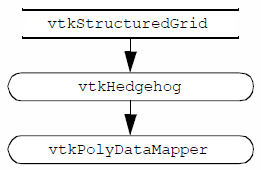
\includegraphics[width=0.8\linewidth]{Figure5-19a}
		\caption*{}
		\label{fig:Figure5-19a}
	\end{subfigure}
	\hfill
	\begin{subfigure}[h]{0.48\linewidth}
		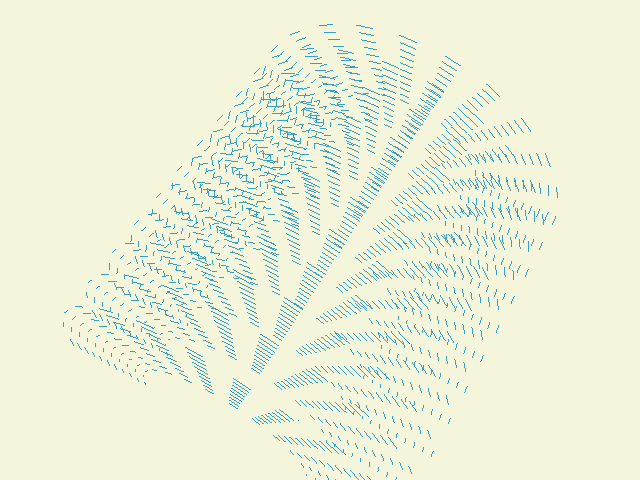
\includegraphics[width=0.8\linewidth]{Figure5-19b}
		\caption*{(\href{https://lorensen.github.io/VTKExamples/site/Cxx/StructuredGrid/SGrid/}{SGrid.cxx} or \href{https://lorensen.github.io/VTKExamples/site/Python/StructuredGrid/SGrid/}{SGrid.py})}
		\label{fig:Figure5-19b}
	\end{subfigure}
	\hfill
	\begin{subfigure}[h]{0.96\linewidth}
		\caption*{}
	\end{subfigure}
	\hfill
	\begin{subfigure}[h]{0.96\linewidth}
		\begin{lstlisting}[language=C++, caption={}]
		vtkStructuredGrid *sgrid = vtkStructuredGrid::New();
		  sgrid->SetDimensions(dims);
		vtkPoints *points = vtkPoints::New();
		  points->Allocate(dims[0]*dims[1]*dims[2]);
		vtkFloatArray *vectors = vtkFloatArray::New();
		  vectors->SetNumberOfComponents(3);
		  vectors->SetNumberOfTuples(dims[0]*dims[1]*dims[2]);
		  deltaZ = 2.0 / (dims[2]-1);
		  deltaRad = (rMax-rMin) / (dims[1]-1);
		  v[2]=0.0;
		  for ( k=0; k<dims[2]; k++)
		    {
		    x[2] = -1.0 + k*deltaZ;
		    kOffset = k * dims[0] * dims[1];
		    for (j=0; j<dims[1]; j++)
		      {
		      radius = rMin + j*deltaRad;
		      jOffset = j * dims[0];
		      for (i=0; i<dims[0]; i++)
		        {
		        theta = i * 15.0 * math.DegreesToRadians();
		        x[0] = radius * cos(theta);
		        x[1] = radius * sin(theta);
		        v[0] = -x[1];
		        v[1] = x[0];
		        offset = i + jOffset + kOffset;
		        points->InsertPoint(offset,x);
		        vectors->InsertTuple(offset,v);
		        }
		      }
		    }
		sgrid->SetPoints(points);
		points->Delete();
		sgrid->GetPointData()->SetVectors(vectors);
		vectors->Delete();
		\end{lstlisting}
		\caption*{}
		\label{fig:Figure5-19c}
	\end{subfigure}
	\caption{Creating a structured grid dataset of a semicylinder. Vectors are created whose magnitude is proportional to radius and oriented in tangential direction.}\label{fig:Figure5-19}
\end{figure}

We arbitrarily choose the number of points in the tangential direction to be thirteen, the number of points in the radial direction to be eleven, and the number of points in the axis direction to be eleven (i.e., dimensions are $13 \times 11 \times 11$ ).

Vectors are generated tangential to the cylinder and of magnitude proportional to the radius. To display the data we draw small, oriented lines at each point as shown in Figure \ref{fig:Figure5-19}. (This technique is called a hedgehog. See ``Hedgehogs and Oriented Glyphs'' on page \pageref{subsec:hedgehogs_oriented_glyphs} for more information.)

The creation of a structured grid dataset is partially explicit and partially implicit. Geometry is created explicitly be creating an instance of vtkPoints, while the topology is created implicitly by specifying dataset dimensions. If the name of the instance of vtkStructuredGrid is sgrid, the following three steps are used to create it.

\begin{itemize}

	\item Specify the dataset geometry by creating an instance of vtkPoints.Use the operators grid->SetPoints() to associate the points with the dataset.

	\item The dataset topology is specified using the operators grid->SetDimensions(). Make sure the number of points created in item number 1 above is equal to the implied number of points $n_x⋅n_y⋅n_z$.

	\item Create point and/or cell attribute data and associate it with the dataset.

\end{itemize}

The topological dimension of the dataset is implied by the specified dimensions. For example, if any of the dimensions $(n_x, n_y, n_z)$ is equal to one, the topological dimension of the dataset is two. If two of the three dimensions $(n_x, n_y, n_z)$ are equal to one, the topological dimension of the dataset is one.

\subsubsection{Create a Rectilinear Grid Dataset}

A rectilinear grid is regular in topology and semi-regular in geometry. Similar to a structured grid or image data dataset, topology is implicitly represented by specifying grid dimensions. Because the grid is axis-aligned but the point coordinates along each axis may vary, we need three data arrays to represent the geometry of the dataset, one array for each of the x-y-z axes. Note that the cell types of the rectilinear dataset are pixels and voxels.

\begin{figure}[!htb]
	\begin{subfigure}[h]{0.48\linewidth}
		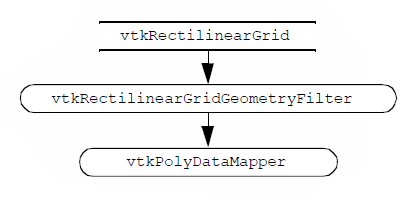
\includegraphics[width=0.96\linewidth]{Figure5-20a}
		\caption*{}
		\label{fig:Figure5-20a}
	\end{subfigure}
	\hfill
	\begin{subfigure}[h]{0.48\linewidth}
		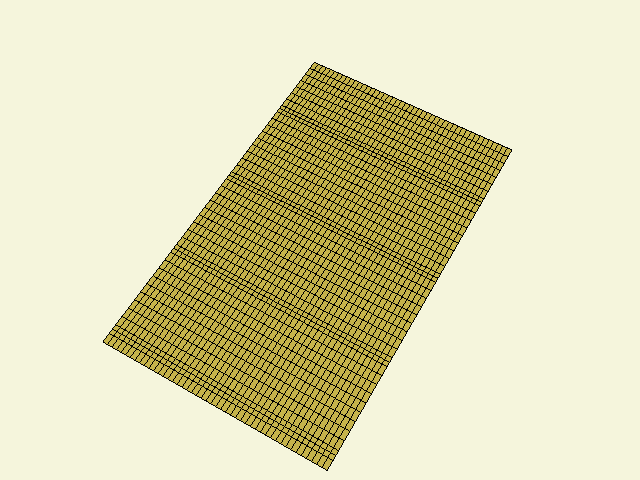
\includegraphics[width=0.96\linewidth]{Figure5-20b}
		\caption*{(\href{https://lorensen.github.io/VTKExamples/site/Cxx/RectilinearGrid/RGrid/}{RGrid.cxx} or \href{https://lorensen.github.io/VTKExamples/site/Python/RectilinearGrid/RGrid/}{RGrid.py})}
		\label{fig:Figure5-20b}
	\end{subfigure}
	\hfill
	\begin{subfigure}[h]{0.96\linewidth}
		\caption*{}
	\end{subfigure}
	\hfill
	\begin{subfigure}[h]{0.96\linewidth}
		\begin{lstlisting}[language=C++, caption={}]
		vtkFloatArray *xCoords = vtkFloatArray::New();
		  for (i=0; i<47; i++) xCoords->InsertNextValue(i,x[i]);
		vtkFloatArray *yCoords = vtkFloatArray::New();
		  for (i=0; i<33; i++) yCoords->InsertNextValue(i,y[i]);
		vtkFloatArray *zCoords = vtkFloatArray::New();
		  for (i=0; i<44; i++) zCoords->InsertNextValue(i,z[i]);
		vtkRectilinearGrid *rgrid = vtkRectilinearGrid::New();
		  rgrid->SetDimensions(47,33,44);
		  rgrid->SetXCoordinates(xCoords);
		  rgrid->SetYCoordinates(yCoords);
		  rgrid->SetZCoordinates(zCoords);
		vtkRectilinearGridGeometryFilter *plane =
		    vtkRectilinearGridGeometryFilter::New();
		  plane->SetInput(rgrid);
		  plane->SetExtent(0,46, 16,16, 0,43);
		vtkPolyDataMapper *rgridMapper = vtkPolyDataMapper::New();
		  rgridMapper->SetInputConnection(plane->GetOutputPort());
		vtkActor *wireActor = vtkActor::New();
		  wireActor->SetMapper(rgridMapper);
		  wireActor->GetProperty()->SetRepresentationToWireframe();
		  wireActor->GetProperty()->SetColor(0,0,0);
		\end{lstlisting}
		\caption*{}
		\label{fig:Figure5-20c}
	\end{subfigure}
	\caption{Creating a rectilinear grid dataset. The coordinates along each axis are defined using an instance of vtkDataArray.}\label{fig:Figure5-20}
\end{figure}

For maximum flexibility when creating rectilinear grids, in VTK we use three vtkDataArray objects to define the axes arrays. This means that different native data type (e.g., unsigned char, int, float, and so on) can be used for each axes.

To summarize the process of creating an instance of vtkRectilinearGrid, we follow four steps. In this example (shown in Figure \ref{fig:Figure5-20}), we assume that the name of the vtkRectilinearGrid instance is rgrid.

\begin{itemize}

	\item Create the dataset geometry by creating three instances of vtkDataArray, one for each of the $x-y-z$ coordinate axes. We will assume that the number of values in each scalar is $n_x$, $n_y$, and $n_z$.

	\item Each of the three instances is assigned to the x, y,and z axes using ther grid->SetXCoordinates(), rgrid->SetYCoordinates(), and rgrid->SetZCoordinates() methods, respectively.

	\item The dataset topology is specified using the operatorr grid->SetDimensions(). Make sure the number of points created in item number 1 above is equal to the implied number of points $n_x⋅n_y⋅n_z$.

	\item Create point and/or cell attribute data and associate it with the dataset.

\end{itemize}

The topological dimension of the dataset is implied by the specified dimensions. For example, if any of the dimensions $(n_x, n_y, n_z)$ is equal to one, the topological dimension of the dataset is two. If two of the three dimensions $(n_x, n_y, n_z)$ are equal to one, the topological dimension of the dataset is one.

\subsubsection{Create an Unstructured Grid Dataset}

Unstructured grid datasets are the most general dataset type in both topology and geometry. In this example we ``artificially'' create an unstructured grid using an instance of vtkUnstructuredGrid (Figure \ref{fig:Figure5-21}). The grid contains examples of each cell type except for pixels and voxels. (Pixels and voxels are generally used internally to process image data datasets. They can be explicitly created and manipulated as long as the required relationship of point geometry is observed.) Creating the dataset structure requires creating points to define the geometry and various cells to define the topology. (Note that in the finite element world we would refer to these as nodes and elements.)

\begin{figure}[!htb]
	\begin{subfigure}[h]{0.48\linewidth}
		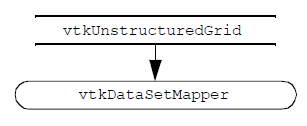
\includegraphics[width=0.96\linewidth]{Figure5-21a}
		\caption*{}
		\label{fig:Figure5-21a}
	\end{subfigure}
	\hfill
	\begin{subfigure}[h]{0.48\linewidth}
		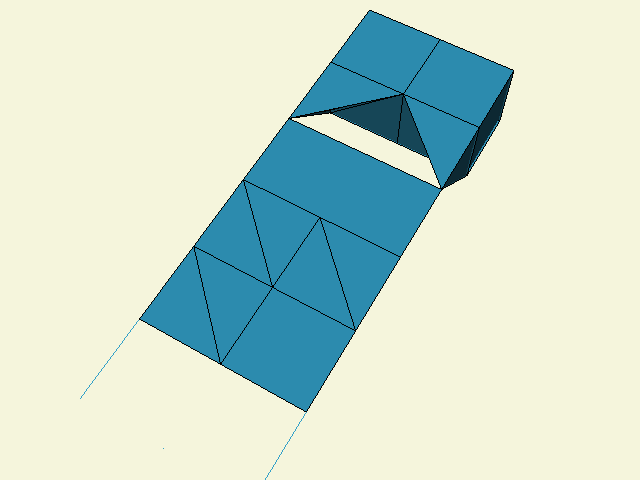
\includegraphics[width=0.96\linewidth]{Figure5-21b}
		\caption*{(\href{https://lorensen.github.io/VTKExamples/site/Cxx/UnstructuredGrid/UGrid/}{UGrid.cxx} or \href{https://lorensen.github.io/VTKExamples/site/Python/UnstructuredGrid/UGrid/}{UGrid.py})}
		\label{fig:Figure5-21b}
	\end{subfigure}
	\hfill
	\begin{subfigure}[h]{0.96\linewidth}
		\caption*{}
	\end{subfigure}
	\hfill
	\begin{subfigure}[h]{0.96\linewidth}
		\begin{lstlisting}[language=C++, caption={}]
		vtkPoints *points = vtkPoints::New();
		  for (i=0; i<27; i++) points->InsertPoint(i,x[i]);
		vtkUnstructuredGrid *ugrid = vtkUnstructuredGrid::New();
		  ugrid->Allocate(100);
		  ugrid->InsertNextCell(VTK_HEXAHEDRON, 8, pts[0]);
		  ugrid->InsertNextCell(VTK_HEXAHEDRON, 8, pts[1]);
		  ugrid->InsertNextCell(VTK_TETRA, 4, pts[2]);
		  ugrid->InsertNextCell(VTK_TETRA, 4, pts[3]);
		  ugrid->InsertNextCell(VTK_POLYGON, 6, pts[4]);
		  ugrid->InsertNextCell(VTK_TRIANGLE_STRIP, 6, pts[5]);
		  ugrid->InsertNextCell(VTK_QUAD, 4, pts[6]);
		  ugrid->InsertNextCell(VTK_TRIANGLE, 3, pts[7]);
		  ugrid->InsertNextCell(VTK_TRIANGLE, 3, pts[8]);
		  ugrid->InsertNextCell(VTK_LINE, 2, pts[9]);
		  ugrid->InsertNextCell(VTK_LINE, 2, pts[10]);
		  ugrid->InsertNextCell(VTK_VERTEX, 1, pts[11]);
		  ugrid->SetPoints(points);
		  points->Delete();
		\end{lstlisting}
		\caption*{}
		\label{fig:Figure5-21c}
	\end{subfigure}
	\caption{Creation of an unstructured grid.}\label{fig:Figure5-21}
\end{figure}

To summarize the process of creating an instance of vtkUnstructuredGrid, we follow five steps. We assume the name of vtkUnstructuredGrid instance is ugrid.

\begin{itemize}

	\item Allocate memory for the dataset. Use the operator ugrid->Allocate(). This operator takes two optional parameters related to the size of the data. The first is the size of the connectivity list, and the second is the amount to extend storage (if necessary). As a rule of thumb, use the number of cells times the average number of points defining each cell for both parameters. Exact values for these parameters are not important, although the choice may affect performance. If you fail to execute this operation before inserting data, the software will break.

	\item Create an instance of a subclass of vtkPoints to define the dataset geometry. Use the operator ugrid->SetPoints() to associate the points with the dataset.

	\item Create the data set topology on a cell by cell basis by using the cell insertion operator ugrid->InsertNextCell(). There are various flavors of this operator, use the appropriate one.

	\item Create point and/or cell attribute data and associate it with the dataset.

	\item Complete the creation process by executing the ugrid->Squeeze() operator.This operator reclaims any extra memory consumed by the data structures. Although this step is not required, it will return memory resource back to the computer system.

\end{itemize}

\section{Chapter Summary}

A dataset represents visualization data. The dataset has an organizing structure, with topological and geometric components, and associated attribute data. The structure of a dataset consists of cells (topology) and points (geometry). An important characteristic of the structure is whether its geometry and topology are regular or irregular (or equivalently, structured or unstructured). Regular data is more compact and usually more computationally efficient than irregular data. However, irregular data is more flexible in representation capability than regular data.

Important dataset types include polygonal data, rectilinear grid, image data, structured grids, and unstructured grids. The polygonal dataset type is used to represent graphics data, as well as many kinds of visualization data. The unstructured grid is the most general type, consisting of arbitrary combinations of all possible cell types.

Attribute data consists of scalars, vectors, tensors, texture coordinates, and normals. Other arrays may also be includes as part of attribute data since it is a type of field data. In the Visualization Toolkit, attribute data is associated with both the dataset point and cells.

\section{Bibliographic Notes}

A variety of representation schemes have been proposed for each dataset type described here. These schemes vary depending on design goals. For example, even the simple volume representation has been implemented with other more complex schemes such as run-length encoding and octrees \cite{Bloomenthal88}. A description of more general representation schemes is available in \cite{Haber91}, the AVS field model \cite{AVS89}, and the compact cell structure \cite{Schroeder94}. An overview of dataset types can be found in \cite{Gelberg90}. Some structures for those mathematically oriented can be found in \cite{Brisson90} and \cite{Poluzzi93}. Haimes \cite{VISUAL3} describes an efficient data structure for unstructured grid visualization.

If you are interested in more details on finite element methods see the classic Zienkiewicz \cite{Zienkiewicz87} or \cite{Gallagher75}. Information about both finite difference and finite element methods is available in \cite{Lapidus82}.

\printbibliography


\section{Exercises}

\begin{enumerate}

\item Consider a pixmap of dimensions 1002. Compare the memory requirements to represent this data using:

\begin{enumerate}

	\item an image dataset,

	\item a structured grid dataset,

	\item a polygonal mesh of quadrilaterals,

	\item an unstructured grid of quadrilateral cells,

	\item and a triangle strip mesh of 100 strips of 200 triangles each.

\end{enumerate}

\item Consider a volume of dimensions 1003. Compare the memory requirements to represent this data using:

\begin{enumerate}

	\item an image dataset,

	\item a structured grid dataset,

	\item and an unstructured grid of hexahedral cells.

\end{enumerate}

\item Develop a representational scheme for a rectilinear grid. How does this compare (in memory requirement) to a structured grid?

\item Consider a volume of dimensions 1003. Compute the memory requirements for the following point attribute types:

\begin{enumerate}

	\item unsigned character scalars (1 byte per scalar),

	\item float scalars (4 bytes per scalar),

	\item float vectors,

	\item and double-precision tensors ($3 \times 3$ tensors).

\end{enumerate}

\item List three examples of scalar data.

\item List three examples of vector data.

\item List three examples of tensor data.

\item Is it possible to have more than one scalar field in a dataset? If so, how would this information be represented?

\item  A common method to represent cell connectivity is to list point ids with the last id negated. For example, triangle $(8,7,3)$ would be represented $(8,7,-3)$. The negative index represents end of cell definition. What are the advantages and disadvantages of this scheme as compared to the VTK cell array structure?

\item  How many different ways can a hexahedral cell be decomposed into tetrahedron? Are there compatibility issues between neighboring hexahedra?

\item Write a program to create and display a structured grid in the form of a hollow cylinder (i.e., cylinder with a hole through it).

\item Write a program to create and display an unstructured grid in the form of a hollow cylinder.

\item Write a program to create and display a polygonal octahedron.

\end{enumerate}
